% !TeX TXS-program:compile = txs:///lualatex/[--shell-escape]
\documentclass[ut8x, 14pt, oneside, a4paper]{extarticle}

\usepackage{mathtext}
\usepackage{amsmath}
\usepackage{amsfonts}
\usepackage{amssymb}
\usepackage[russian]{babel}
\usepackage{latexsym}
\usepackage{indentfirst}
\usepackage{mathtools}
\usepackage{graphicx}
\usepackage{csvsimple}
\graphicspath{}
\DeclareGraphicsExtensions{.pdf,.png,.jpg, .eps, .svg}
\usepackage[top=20mm, right = 10mm, left = 30mm, bottom = 20mm]{geometry}
\linespread{1.3}
\usepackage{color} 
\usepackage{listings} 
\usepackage{pythonhighlight}
\usepackage{caption}
\usepackage{ragged2e}
\justifying

\usepackage{amsmath}

\usepackage{setspace}
\onehalfspacing % Полуторный интервал

\frenchspacing
\usepackage{indentfirst} % Красная строка

\usepackage{titlesec}
\titleformat{\section}
{\normalsize\bfseries}
{\thesection}
{1em}{}
\titlespacing*{\section}{\parindent}{*4}{*4}
\titlespacing*{\subsection}{\parindent}{*4}{*4}

\usepackage{titlesec}
%\titleformat{\section}{\Large\bfseries}{\thesection}{20pt}{\Large\bfseries}

\titleformat{name=\section}[block]
{\normalfont\Large\bfseries\hspace{\parindent}}
{\thesection}
{1em}
{}
\titleformat{name=\section,numberless}[block]
{\normalfont\Large\bfseries\centering}
{}
{0pt}
{}

\newcommand{\anonsection}[1]{%
	\section*{\centering#1}%
	\addcontentsline{toc}{section}{#1}%
}
\usepackage[figurename=Рисунок]{caption}
\usepackage{placeins}

\usepackage{caption}
\captionsetup{justification=raggedright,singlelinecheck=false}
\addto\captionsrussian{\def\refname{Список использованных источников}}
\usepackage{url}

\usepackage{cmap} % Улучшенный поиск русских слов в полученном pdf-файле
\usepackage{fontspec}
\usepackage{pdfpages}

\usepackage[square,numbers,sort&compress]{natbib}
\renewcommand{\bibnumfmt}[1]{#1.\hfill}
\setmainfont{Times New Roman}

\makeatletter
\renewenvironment{thebibliography}[1]
{\section*{\bibname}% <-- this line was changed from \chapter* to \section*
	\@mkboth{\MakeUppercase\bibname}{\MakeUppercase\bibname}%
	\list{\@biblabel{\@arabic\c@enumiv}}%
	{\settowidth\labelwidth{\@biblabel{#1}}%
		\leftmargin\labelwidth
		\advance\leftmargin\labelsep
		\@openbib@code
		\usecounter{enumiv}%
		\let\p@enumiv\@empty
		\renewcommand\theenumiv{\@arabic\c@enumiv}}%
	\sloppy
	\clubpenalty4000
	\@clubpenalty \clubpenalty
	\widowpenalty4000%
	\sfcode`\.\@m}
{\def\@noitemerr
	{\@latex@warning{Empty `thebibliography' environment}}%
	\endlist}
\makeatother

\begin{document}
	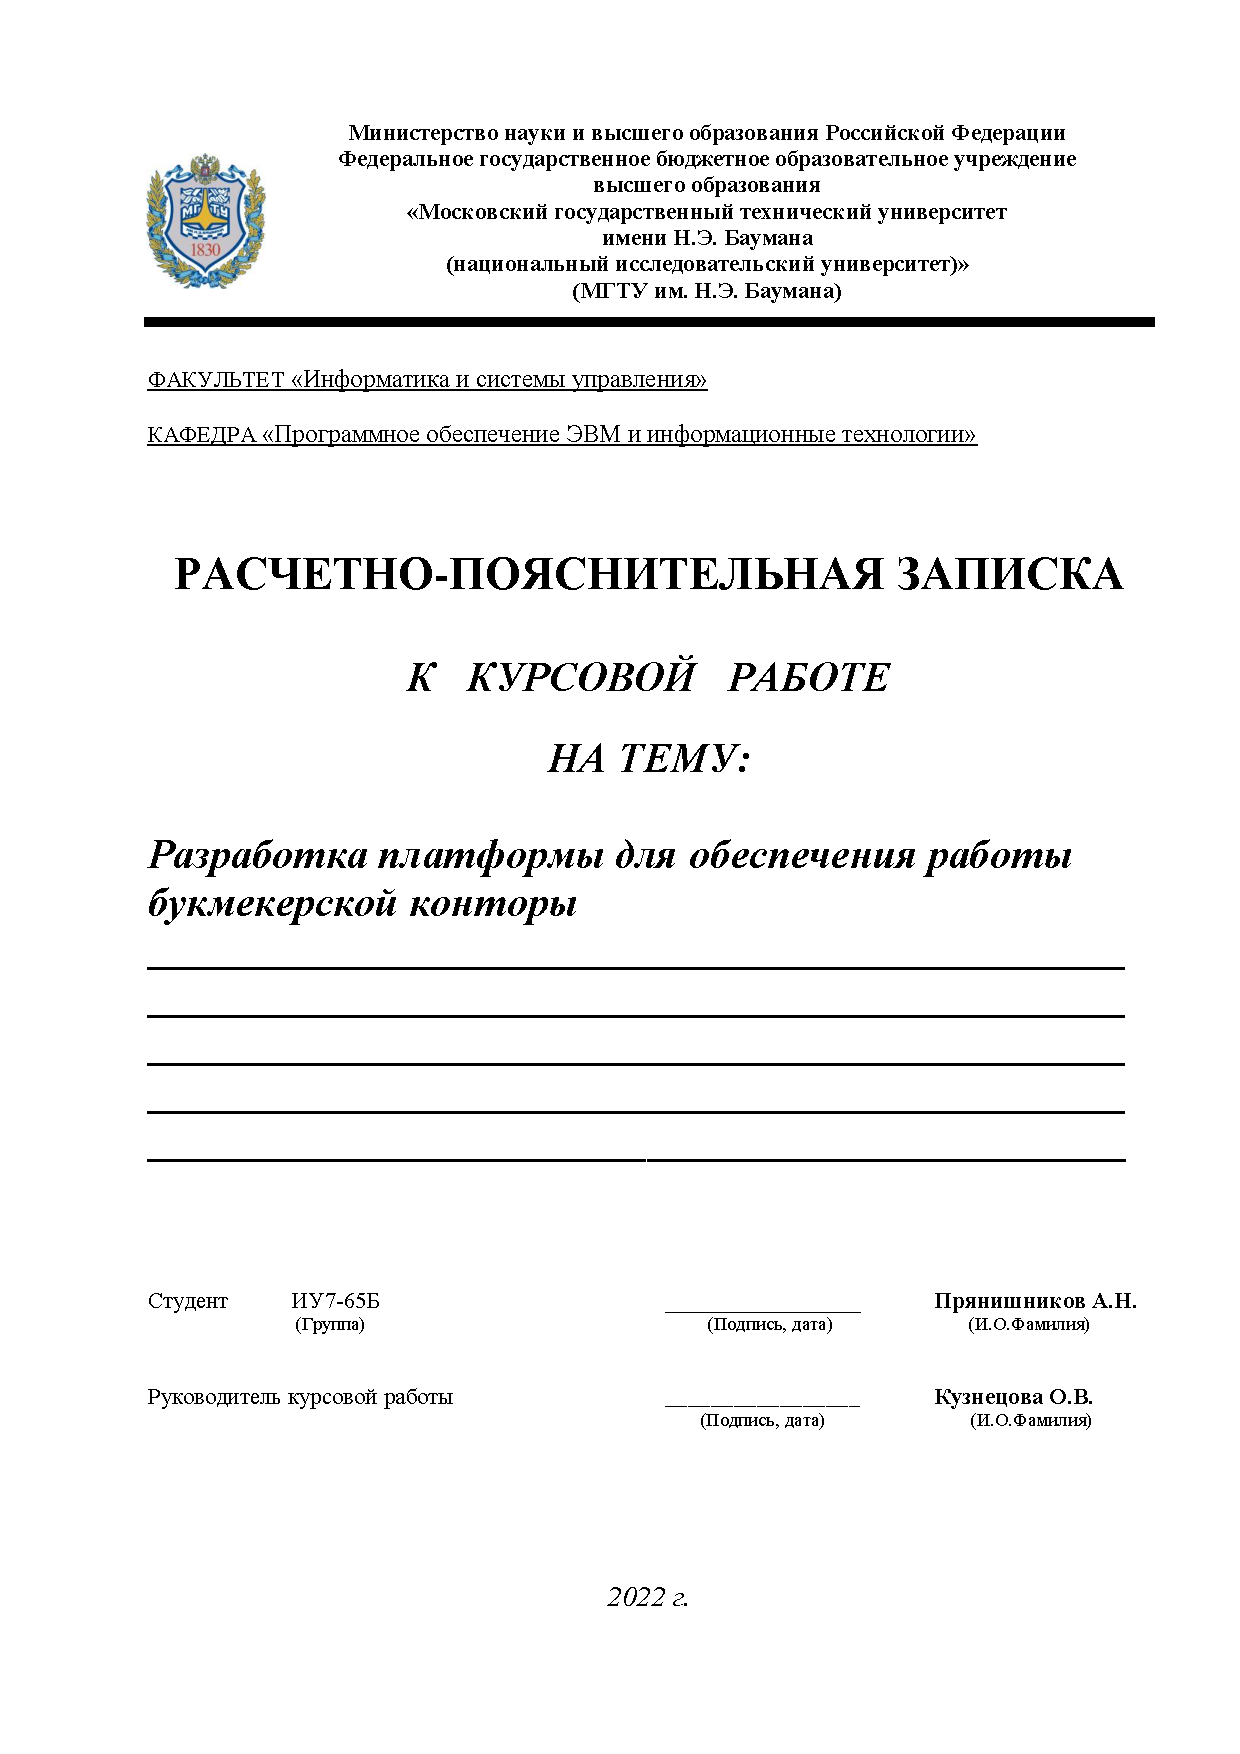
\includepdf[pages=-]{title.pdf}
	\setmainfont{Times New Roman}
	\anonsection{РЕФЕРАТ}

Расчетно-пояснительная записка 48 с., 16 рис., 1 табл., 10 ист.

В работе представлена разработка платформы для обеспечения работы букмекерской конторы.

Проведена формализация задачи и определён требуемый функционал. Проведён анализ предметной области и описана структура БД. 
Спроектировано приложения для доступа к БД. Создана и заполнена база данных. Разработан понятный интерфейс для клиента. 
Разработано ПО, позволяющее пользователям совершать интерактивные ставки на различные события в букмекерской конторе.
Проведено исследование времени ответа БД от индексации.

КЛЮЧЕВЫЕ СЛОВА

\textit{База данных, PostgreSQL, Букмекерская контора, Qt, Python}

\pagebreak
	\def\contentsname{СОДЕРЖАНИЕ}
	\tableofcontents
	\anonsection{ВВЕДЕНИЕ}
Букмекерская контора -- игорное заведение, в котором организатор азартных игр заключает пари с участниками данного вида азартных игр. 

Букмекерские конторы имеют огромное влияние на спорт: они заключают крупные спонсорские контракты с соревнованиями и клубами, вовлекают большое количество болельщиков к просмотру матчей, а также проводят собственные турниры. 

Актуальность работы состоит в том, что букмекерская контора требует постоянного взаимодействия с базой данных, которую требуется эффективно спроектировать.

Цель курсовой работы: разработать платформу для обеспечения работы букмекерской конторы, в которой пользователи могут заключать пари на виртуальные события.

Для достижения поставленной цели требуется выполнить следующие задачи:
\begin{enumerate}
	\item Провести формализацию задачи и определить требуемый функционал.
	\item Провести анализ предметной области и описать структуру БД, включая объекты, из которых она состоит.
	\item Спроектировать приложение для доступа к БД.
	\item Создать и заполнить БД.
	\item Реализовать понятный интерфейс для клиента.
	\item Разработать ПО, позволяющее пользователям совершать интерактивные ставки на различные события в букмекерской конторе.
\end{enumerate} 

	
	\chapter{Аналитический раздел}
В этом разделе будут рассмотрены определения букмекерской конторы, принципы её функционирования и требования к базе данных, обеспечивающих её работу.

\section{Основные определения}
В статье 4 Федерального Закона от 29.12.2006 N 244-ФЗ (ред. от 02.07.2021) "О государственном регулировании деятельности по организации и проведению азартных игр и о внесении изменений в некоторые законодательные акты Российской Федерации" содержатся следующие определения \cite{bk}:

\textbf{Азартная игра} -- основанное на риске соглашение о выигрыше, заключенное двумя или несколькими участниками такого соглашения между собой либо с организатором азартной игры по правилам, установленным организатором азартной игры \cite{bk}.

\textbf{Пари} -- азартная игра, при которой исход основанного на риске соглашения о выигрыше, заключаемого двумя или несколькими участниками пари между собой либо с организатором данного вида азартной игры, зависит от события, относительно которого неизвестно, наступит оно или нет \cite{bk}.

\textbf{Интерактивная ставка} - денежные средства, в том числе электронные денежные средства, передаваемые с использованием электронных средств платежа, в том числе посредством информационно-телекоммуникационных сетей, включая сеть "Интернет" \cite{bk}.

\textbf{Букмекерская контора} - игорное заведение, в котором организатор азартных игр заключает пари с участниками данного вида азартных игр \cite{bk}.

\section{Принцип работы букмекерской конторы}
Букмекерская контора предлагает игрокам заключить пари на различные события. 
Тип событий может быть различным, но почти всегда букмекерская линия представлена спортивными соревнованиями.
Спорт доминирует на рынке, так как является непредсказуемым, матчи происходят каждый день, и по всему миру живёт огромное количество болельщиков.

Букмекерская контора предлагает коэффициенты на возможные исходы события. Например, в случае футбольного матча такими исходами является победа одной из команд или ничья. Игрок имеет возможность заключить с конторой пари на наступление какого-либо исхода, сделав ставку. Если этот исход наступил, то букмекерская контора должна вернуть игроку денежные средства на сумму, умноженную на коэффициент исхода. В противном случае букмекерская контора оставляет сумму ставки у себя \cite{kfs}.

Рассмотрим первое приближение выбора коэффициента. Пусть $p$ - вероятность наступления какого-либо исхода. Тогда коэффициент рассчитывается по формуле \ref{first}: 
\begin{equation}\label{first}
k = \frac{1}{p}
\end{equation}

Пусть $N$ -- количество ставок игрока, а $S$ -- сумма одной ставки. Математическое ожидание заработка игрока можно посчитать по формуле \ref{win}:
\begin{equation}\label{win} 
M = k_1 * S * p * N - S * N = \frac{1}{p} * S * p * N - S * N = 0
\end{equation}

Так как выигрыш букмекера формируется из проигрыша игрока, из \ref{win} следует, что и математическое ожидание заработка букмекера тоже равняется нулю.

Но букмекерская контора рассчитывает зарабатывать и в краткосрочной, и в долгосрочной перспективе. Для получения прибыли в каждом матче в коэффициенты закладывается маржа. Пусть $p_{win}$ - процент маржи, которые контора хочет иметь, а $\omega$ -- количество исходов события. Тогда коэффициент рассчитывается по формуле \ref{second}:
\begin{equation}\label{second}
k = \frac{1}{p + \frac{p_{win}}{\omega}}
\end{equation}

В таком случае математическое ожидание заработка игрока будет отрицательным, так как коэффициент стал меньше, чем в \ref{first}. Исходя из этого, букмекерская контора остаётся в выигрыша при наступлении любого исхода.

Для того, чтобы постоянно зарабатывать, букмекерам требуется безошибочно рассчитывать вероятности наступления всех событий. 
Этим обычно занимаются профессиональные аналитики и статистики.

Теперь рассмотрим событие, в котором есть два противоположных исхода -- выигрыш одной из команд. Пусть $k_1$ и $k_2$ -- коэффициенты на эти исходы, а $S_1$ и $S_2$ -- денежная сумма, поставленная на эти исходы. 
Если реализуется первый исход, то заработок БК составит $S_1 + S_2 - k_1 * S_1$, а если второй исход -- 
$S_1 + S_2 - k_2 * S_2$. 

Денежные потоки могут быть распределены таким образом, что их распределение не будет соответствовать рассчитанным вероятностям наступления событий. 
В таком случае при наступлении одного из событий БК потеряет деньги.
Следовательно, требуется постоянно обновлять коэффициенты, опираясь на объём средств, поставленных игроками на каждый исход.

При этом всём на букмекерском рынке большая конкуренция, следовательно, требуется предлагать самые выгодные коэффициенты на рынке.

Подводя итог, расчёт коэффициентов на матчи -- сложная математическая, экономическая и маркетинговая задача, которая и позволяет букмекерам зарабатывать деньги \cite{kfs}.

\section{Основные роли в букмекерской конторе}
Букмекерская контора заключает пари с игроками, поэтому первая роль, которая требуется -- \textbf{игрок}. 
Для игроков требуется добавить возможность просмотра линии событий, заключения пари, пополнение баланса, изменения личных данных.
При этом нужно добавить регистрацию, чтобы новый игрок мог воспользоваться аккаунтов, только лишь загрузив приложение. 

Согласно закону № 115-ФЗ «О противодействии легализации (отмыванию) доходов, полученных преступным путем, и финансированию терроризма» об азартных играх, букмекерская контора должна обязательно проводить процедуру идентификации клиентов \cite{bk2}. 
Обычно в букмекерских конторах есть администраторы, которые проверяют указанные игроком данные, и верифицируют аккаунтов. 
Лишь после этого у клиента есть возможность совершать ставки на какие-либо события.
Поэтому следующая роль -- \textbf{администратор}.

В его функционал входит верификация новых пользователей или отклонение заявки игрока.
Подразумевается, что администратор имеет доступ к какой-то сторонней базе данных, где может проверить паспортные данные, однако это выходит за пределы курсовой работы.
Поэтому администратор просто имеет возможность изменить статус игрока.

Также в букмекерской конторе кто-то должен заниматься линией матчей. 
Требуется добавлять новые матчи в линию, изменять их статус (событие началось, закончилось), менять текущий счёт и изменять коэффициенты.
Этим занимается \textbf{аналитик}, который имеет возможность добавлять события в линию и менять о них информацию.

Use-Case диаграмма ролей проекта представлена на рисунке 1.1:

\FloatBarrier
\begin{figure}[hp]	
	\begin{center}
		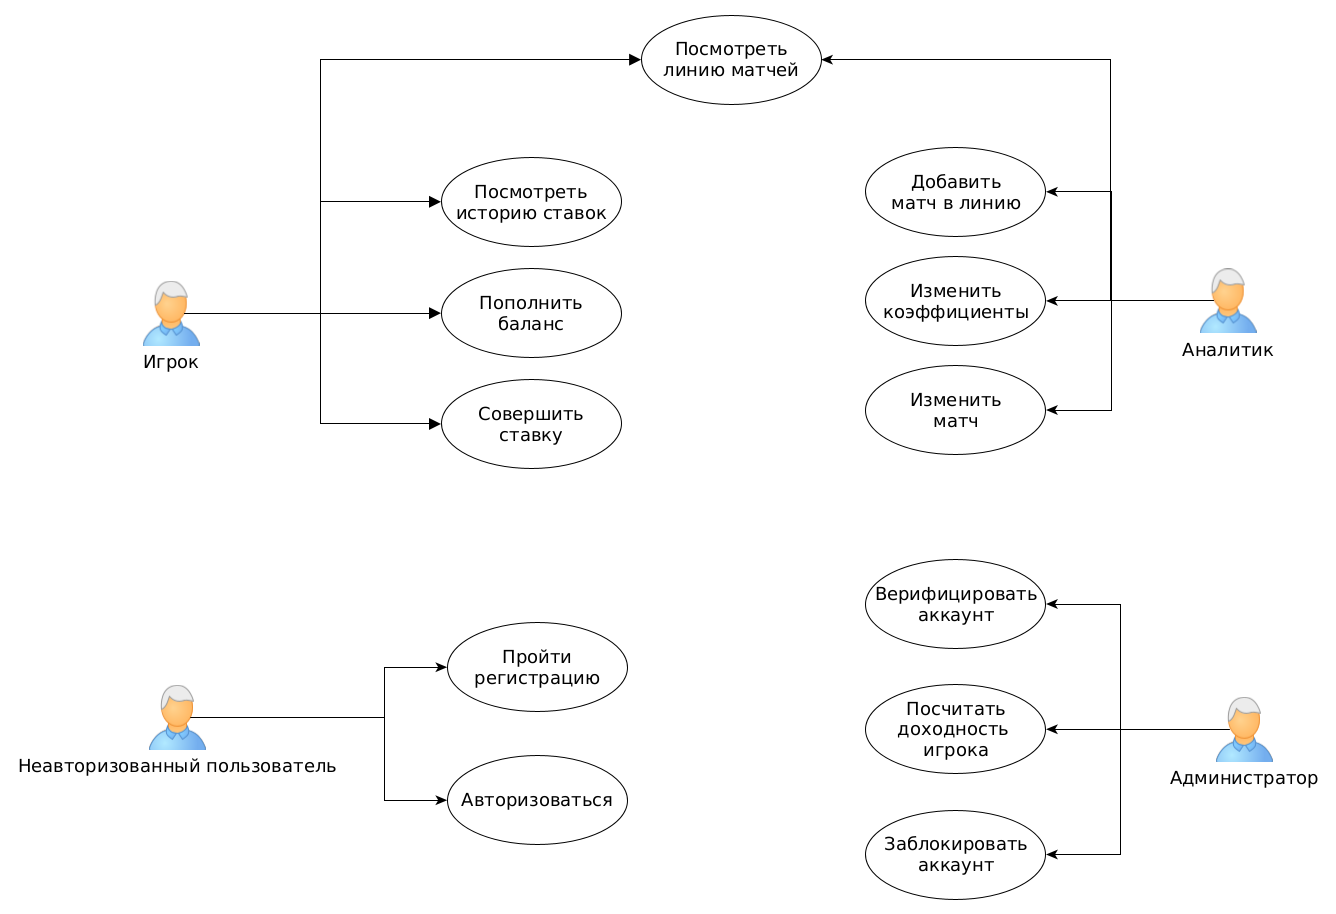
\includegraphics[width=\linewidth]{inc/useCase.png}
	\end{center}
	\caption{Use-Case диаграмма}
	\label{fig::UseCase}
\end{figure}
\FloatBarrier


\section{Цикл одного события в букмекерской конторе}
Для обеспечения работы букмекерской платформы требуется, чтобы игроку был предоставлен выбор из событий.
Требуется, чтобы аналитик добавил событие в букмекерской конторе. 
Событие происходит в абстрактном виде спорта, в котором возможно три исхода: победа первой команды, ничья, и победа второй команды. 
У каждого события есть дата и время начала, две команды, которые встречаются в матче, а также коэффициенты на каждый из исходов.
Аналитик должен указать все данные события. 
Для упрощения работы, список команд должен быть постоянным, и храниться в базе данных. 
При этом в одном событии не может быть двух одинаковых команд, а коэффициенты на исход должны соответствовать теоретическим изложениям из п.1.2 настоящего РПЗ.

У каждого события есть атрибут статуса. Всего есть три варианта:
\begin{enumerate}
	\item Событие запланировано, но ещё не началось.
	\item Событие идёт в текущий момент.
	\item Событие закончилось.
\end{enumerate} 

Аналитику требуется своевременно вносить правки в статус матча: изменять статус события, изменять счёт встречи, а также менять коэффициенты в зависимости от того, как складывается встреча.

Как только аналитик пометил событие законченным, у матча меняется статут на "закончен", и букмекерская контора должна рассчитать тех, кто выиграл пари, и заплатить им.

\section{Требования к базе данных букмекерской конторы}
Платформа для обеспечения работы букмекерской конторы должна использовать базу данных для нескольких целей:
\begin{enumerate}
	\item Хранения информации о пользователях, их балансе и личной информации.
	\item Хранения информации о событиях в линии, причём как запланированных и текущих, так и о законченных.
	\item Хранения информации о совершённых игроком ставок для прозрачности работы конторы.
	\item Автоматического обновления баланса игроков при заключении пари и перерасчёта в случае выигрыша.
	\item Хранения информации об аккаунтах и ролях, связанных с ними.
	\item Различий в возможностях ролей при работе с базой данных.
\end{enumerate}

Также требуется обратить внимание на следующие детали при разработке базы данных:
\begin{itemize}
	\item данные в букмекерской конторе не должны быть избыточны, следовательно, требуется привести отношения к нормальной форме;
	\item букмекерская контора хранит персональные данные пользователей, следовательно, требуется обеспечить безопасность работы с паспортными данными, паролями, чтобы их было невозможно получить нежелательным лицам;
	\item так как состояние матча также хранится в БД, автоматическое обновление баланса игроков можно реализовать при помощи триггеров на определённые события;
	\item ставка может считаться сделанной, если информация о ней записана в БД и с баланса игрока списаны средства, равные размеру ставки. При этом коэффициент может измениться во время работы системы. Поэтому требуется использовать транзакции для поддержки функционала заключения пари.
\end{itemize}

\section{Основные отношения в базе данных}
В соответствии с вышеперечисленными аспектами базы данных для платформы, в БД должны быть представлены следующие отношения с атрибутами:
\begin{enumerate}
	\item \textbf{Аккаунты}. В качестве информации должен храниться логин и пароль для входа в систему, а также роль, соответствующая аккаунту. Это отношение может быть изменено напрямую только администратором. Также оно автоматически обновляется при регистрации нового игрока.
	\item \textbf{Пользователи}. В этом отношении должна храниться основная личная информация о пользователе: номер телефона, электронная почта, номер паспорта. Также оно содержит информацию о балансе игрока и максимальной ставке. Предполагается, что букмекерская контора будет иметь возможность порезать счёт успешного игрока, существенно уменьшив собственные убытки.
	\item \textbf{Команды}. В этом отношении должны храниться команды, которые могут быть в событии. В качестве атрибутов рассматривается название, логотип и город.
	\item \textbf{События}. В этом отношении хранятся все события: дата создания, их статус, итоговый счёт, команды, принимающие участия. 
	\item \textbf{Ставки}. В этом отношении хранятся все совершённые ставки и события.
\end{enumerate}

Концептуально отношения в базе данных можно представить с помощью ER-модели нотации Чена.
На рисунке 1.2 представлена ER-модель в нотации Чена:
\FloatBarrier
\begin{figure}[hp]	
	\begin{center}
		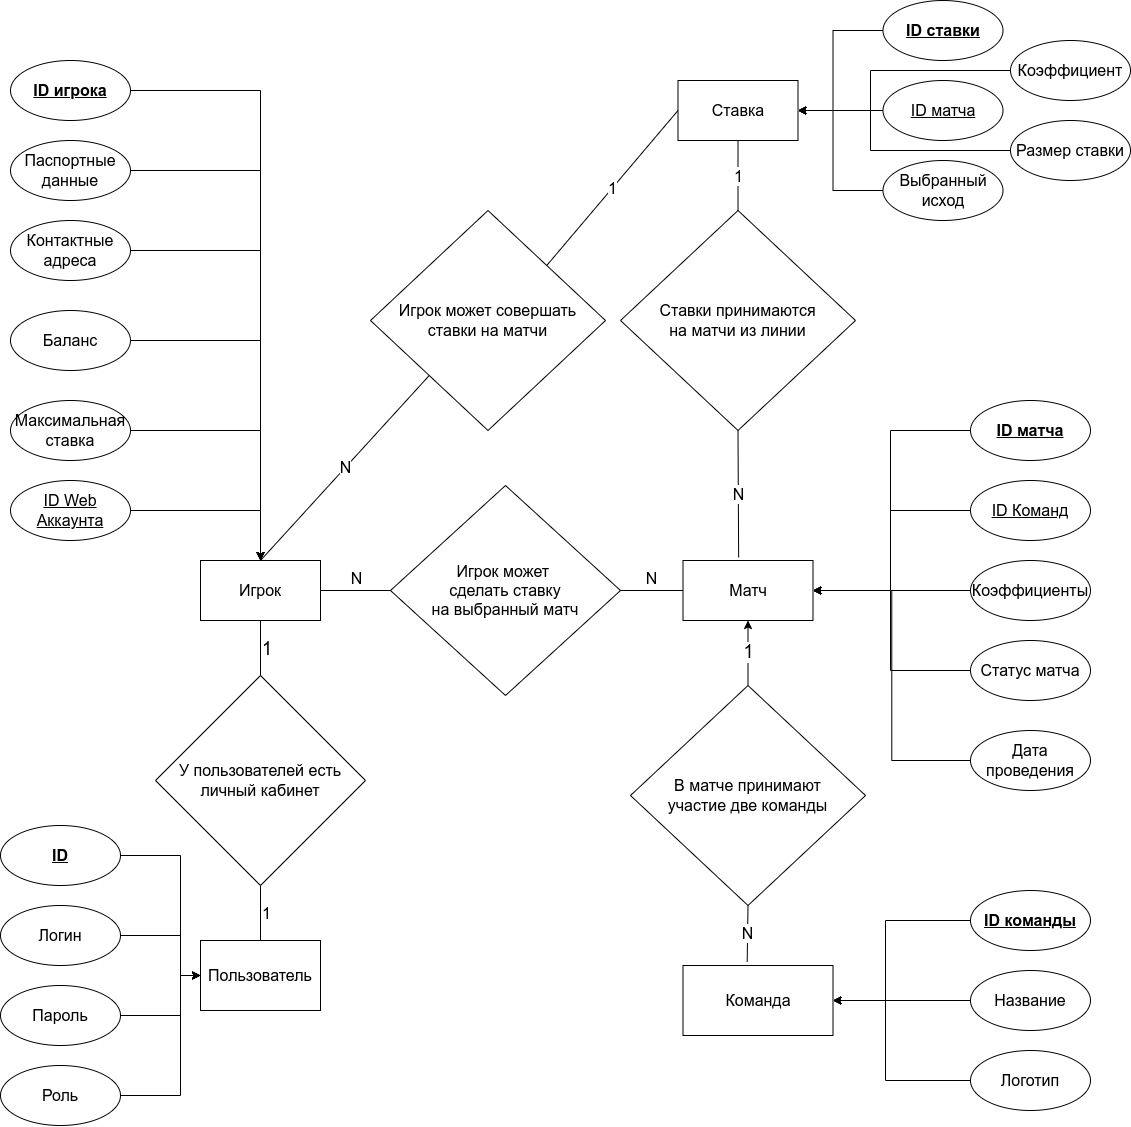
\includegraphics[width=\linewidth]{inc/chen.png}
	\end{center}
	\caption{ER-модель в нотации Чена}
	\label{fig::chen}
\end{figure}
\FloatBarrier

	\section{Конструкторский раздел}
В этом разделе будет проведено проектирование базы данных и приложения, а также приведены схемы разрабатываемых алгоритмов.

\subsection{Проектирование базы данных}
База данных приложения будет реализована с помощью следующих страниц:
\begin{enumerate}
	\item таблица пользователей User;
	\item таблица игроков Account;
	\item таблица команд Teams;
	\item таблица матчей Games;
	\item таблица ставок Bet;
\end{enumerate}

Таблица пользователей \textbf{User} содержит информацию о логинах, паролях аккаунтов, а также о ролях, соответствующих аккаунту.
Содержит следующие поля:
\begin{itemize}
	\item id -- первичный ключ, идентификатор аккаунта;
	\item userLogin -- логин пользователя;
	\item password -- пароль пользователя;
	\item creationDate -- дата регистрации аккаунта;
	\item userRole -- роль, соответствующая аккаунту.
\end{itemize}

Таблица пользователей \textbf{Account} содержит информацию о личности игрока, который совершает ставки в букмекерской конторе.
Содержит следующие поля:
\begin{itemize}
	\item accID -- первичный ключ, идентификатор аккаунта;
	\item userID -- внешний ключ, соответствует идентификаторам интернет аккаунта;
	\item userName -- имя пользователя, указанное при регистрации;
	\item userSurname -- фамилия пользователя, указанное при регистрации;
	\item dateOfBirth -- дата рождения пользователя;
	\item phoneNumber -- номер телефона пользователя;
	\item email -- электронная почта пользователя;
	\item passportNumber -- номер паспорта пользователя;
	\item userStatus -- статус пользователя: на верификации, активный и заблокированный аккаунты;
	\item balance -- текущий баланс пользователя;
	\item maxBet -- размер максимальной ставки, доступной игроку.
\end{itemize}

Таблица команд \textbf{Teams} содержит информацию о командах, которые могут принимать участие в матче.
Содержит следующие поля:
\begin{itemize}
	\item teamID -- первичный ключ, идентификатор команды;
	\item teamName -- название команды;
	\item teamcity -- город, из которого команда;
	\item logo -- локальный путь к картинке эмблемы команды.
\end{itemize}

Таблица матчей \textbf{Games} содержит информацию о матчах, на которые принимаются ставки в букмекерской конторе.
Содержит следующие поля:
\begin{itemize}
	\item gameID -- первичный ключ, идентификатор матча;
	\item gameStatus -- соответствует текущему состоянию матча: запланирован, идёт или закончился;
	\item team1ID -- внешний ключ, соответствует id первой команды;
	\item team2ID -- внешний ключ, соответствует id второй команды;
	\item w1Coef -- текущий коэффициент на победу первой команды;
	\item drawCoef -- текущий коэффициент на ничью;
	\item w2Coef -- текущий коэффициент на победу второй команды;
	\item gameResult -- текущий счёт в матче;
	\item gameDate -- дата проведения матча;
	\item gameTime -- время начала матча;
\end{itemize}

Таблица ставок \textbf{Bet} содержит информацию о совершённых пользователями ставках.
Содержит следующие поля:
\begin{itemize}
	\item betID -- первичный ключ, идентификатор ставки;
	\item gameID -- внешний ключ, соответствует идентификатору матча;
	\item accID -- внешний ключ, соответствует id пользователя, который совершил ставку;
	\item choosedResult -- выбранный результат (0 -- ничья, 1 -- победа первой команды, 2 -- победа второй команды);
	\item betDate -- время совершения ставки;
	\item betSize -- размер совершенной ставки;
	\item koef -- коэффициент, по которому игрок совершил ставку;
	\item betStatus -- текущее состояние ставки: принята, выиграна или проиграна;
	\item payoutAmount -- выплата по результатам совершения события;
\end{itemize}

\newpage

ER-модель БД в нотации Crow’s Foot представлена на рисунке 3:
\FloatBarrier
\begin{figure}[h]	
	\begin{center}
		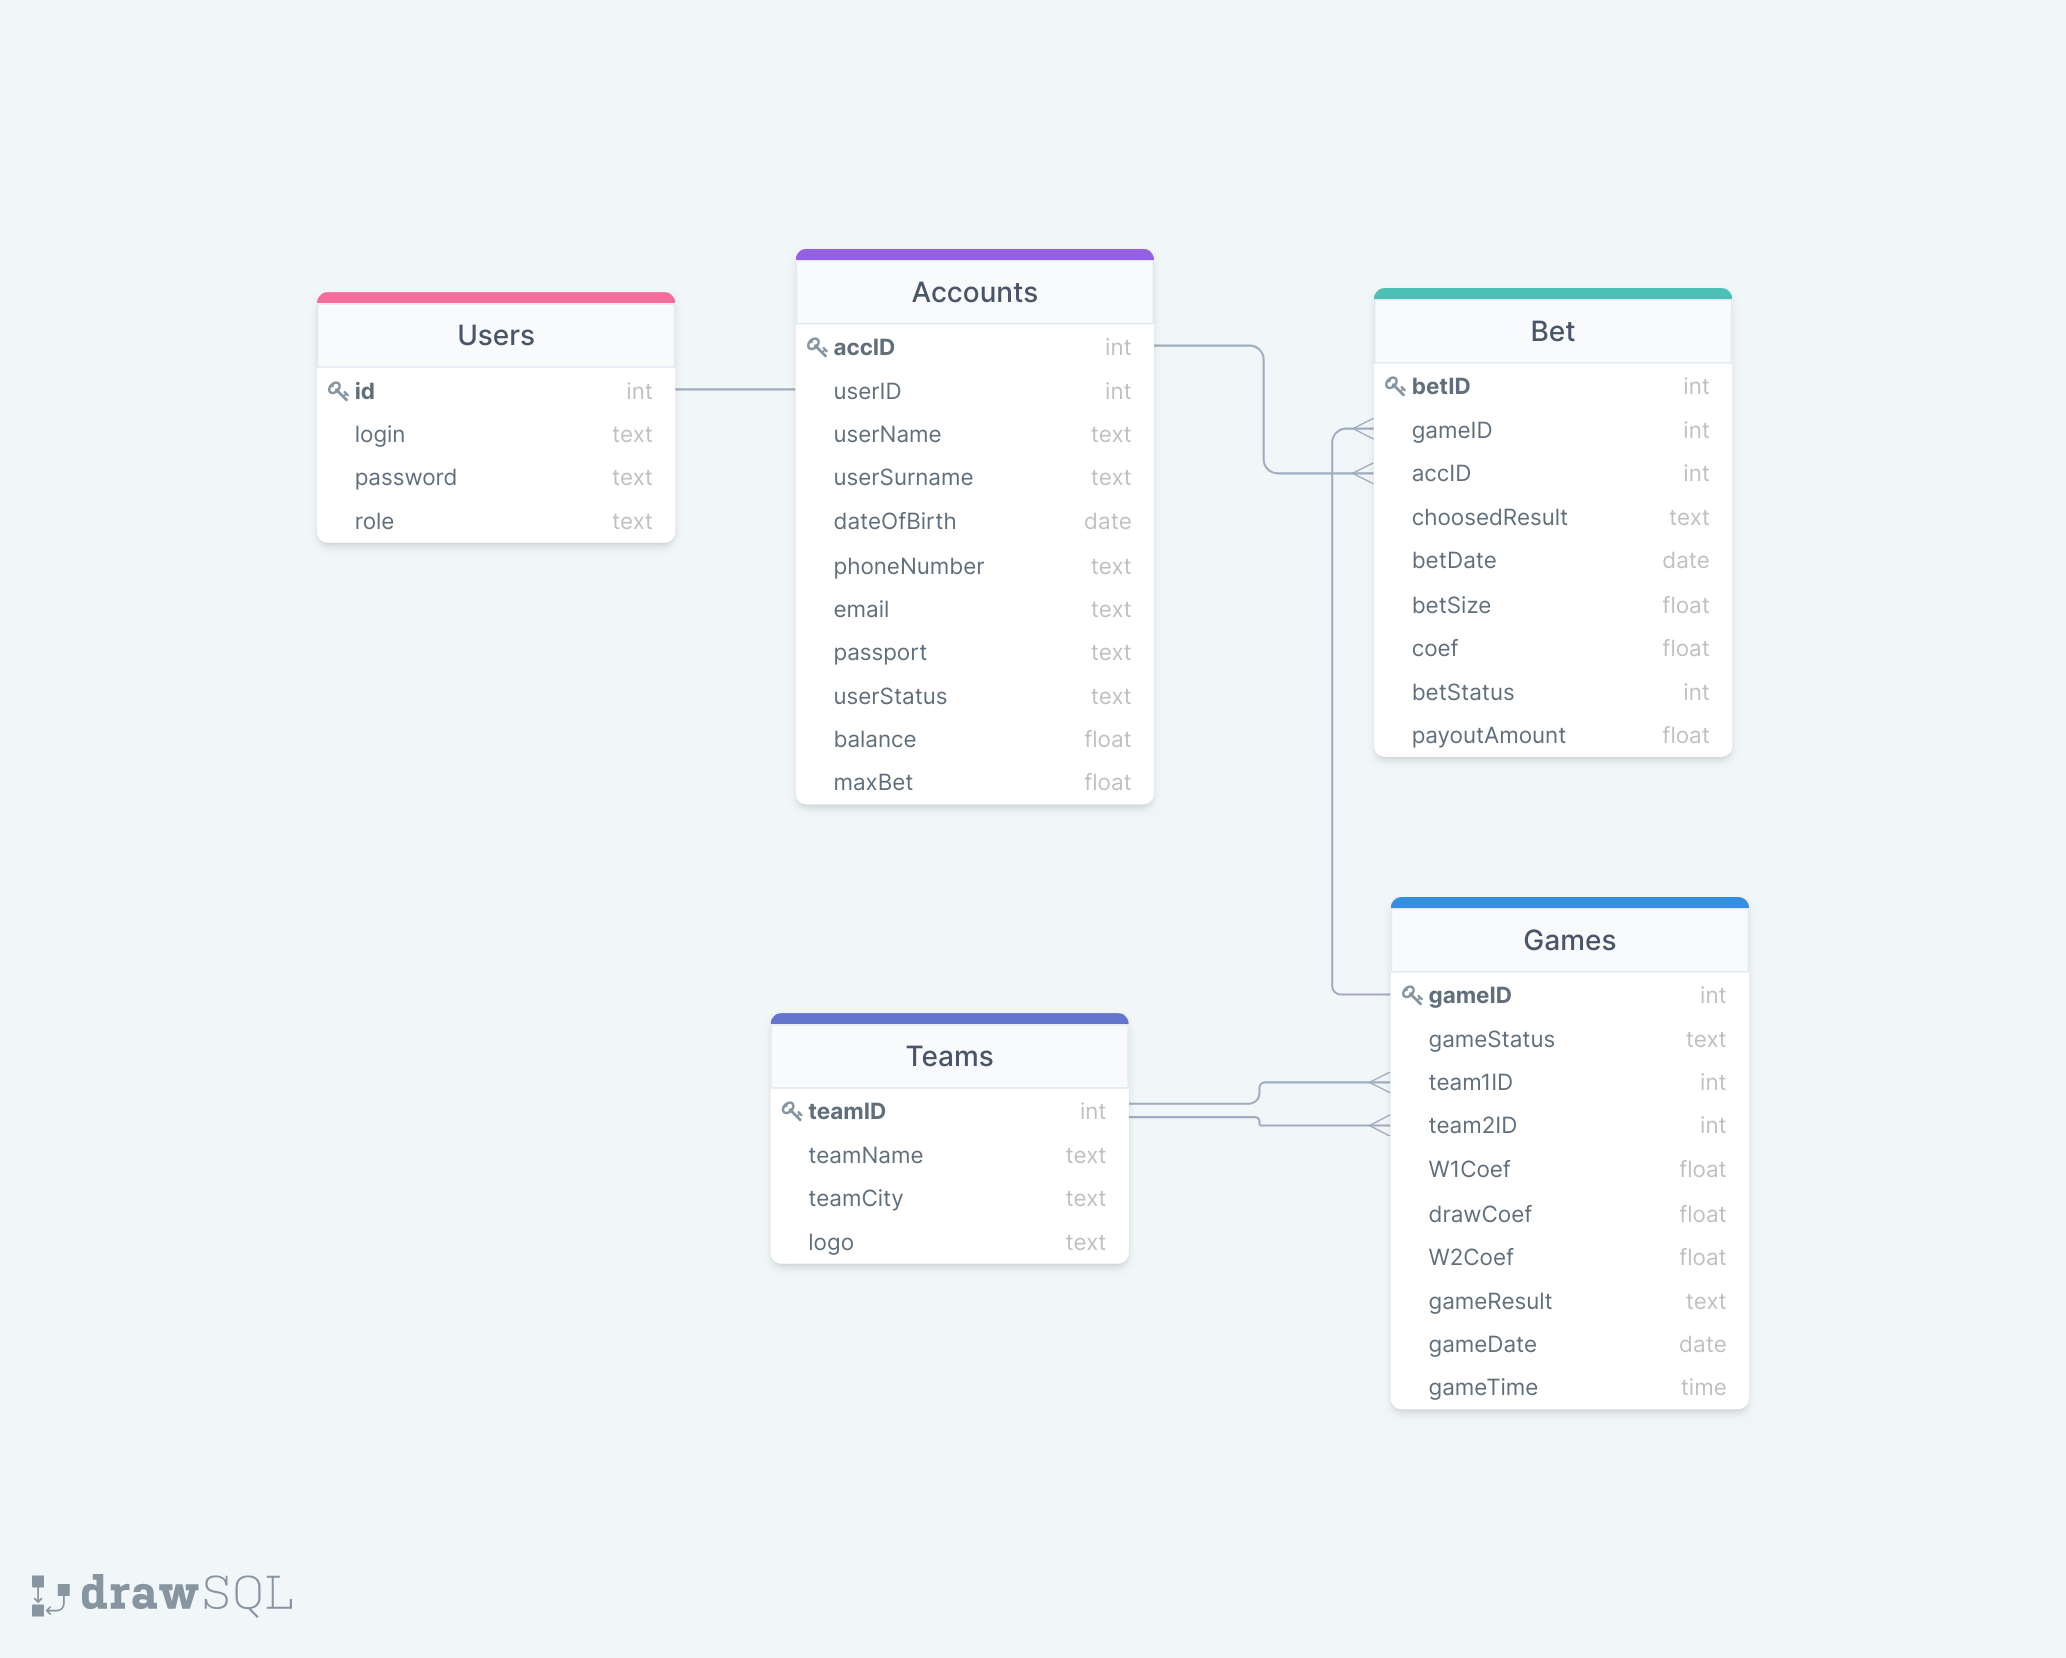
\includegraphics[width=\linewidth]{inc/scheme.png}
	\end{center}
	\caption{ER-модель базы данных в нотации Crow’s Foot}
	\label{fig::scheme}
\end{figure}
\FloatBarrier

\subsection{Тип приложения}
Тип приложения был выбран Desktop по двум следующим причинам:
\begin{enumerate}
	\item Реальные букмекерские конторы разрабатывают версии программного обеспечения для ПК, так как это позволяет пользователям удобнее и быстрее взаимодействовать с системой.
	\item Desktop-приложение не предоставляет дополнительных требований к времени ответу системы, как, например, высоконагруженный сервис. 
\end{enumerate}

\subsection{Проектирование приложения}
Структура приложения основана на парадигмах ООП. 

Для реализации работы приложения были реализованы следующие классы:
\begin{itemize}
	\item class UI -- класс содержит функции для загрузки новой страницы формата .ui и создания контроллера под неё;
	\item class Controllers -- набор классов, каждый из которых контролирует связь элементов страниц друг с другом;
	\item class Facade -- класс, является реализацией паттерна «Фасад»;
	\item class Command -- набор классов, являются реализацией паттерна «Команда»;
	\item class AuthManager -- класс, являющийся сущностью между действий в UI и базой данных для неавторизованного пользователя;
	\item class PlayerManager -- класс, являющийся сущностью между действий в UI и базой данных для вошедшего в систему игрока;
	\item class AdminManager -- класс, являющийся сущностью между действий в UI и базой данных для администратора БК;
	\item class AnalyzerManager -- класс, являющийся сущностью между действий в UI и базой данных для аналитика;
	\item class AuthRepo -- класс, непосредственно взаимодействующий с базой данных для неавторизованного пользователя; 
	\item class PlayerRepo -- класс, непосредственно взаимодействующий с базой данных для авторизованного игрока; 
	\item class AdminRepo -- класс, непосредственно взаимодействующий с базой данных для администратора БК; 
	\item class AnalyzerRepo -- класс, непосредственно взаимодействующий с базой данных для аналитика; 
	\item class SessionHolder -- класс, реализующий паттерн «Прокси», выполняющий хэширование данных текущего игрока. Позволяет не взаимодействовать с БД для получения данных пользователя;
	\item class ValidateManager -- набор классов, валидующих данные: при регистрации, при добавлении нового матча или корректировке коэффициентов.
\end{itemize}

На рисунке 4 представлена UML-диаграмма классов.
\FloatBarrier
\begin{figure}[h]	
	\begin{center}
		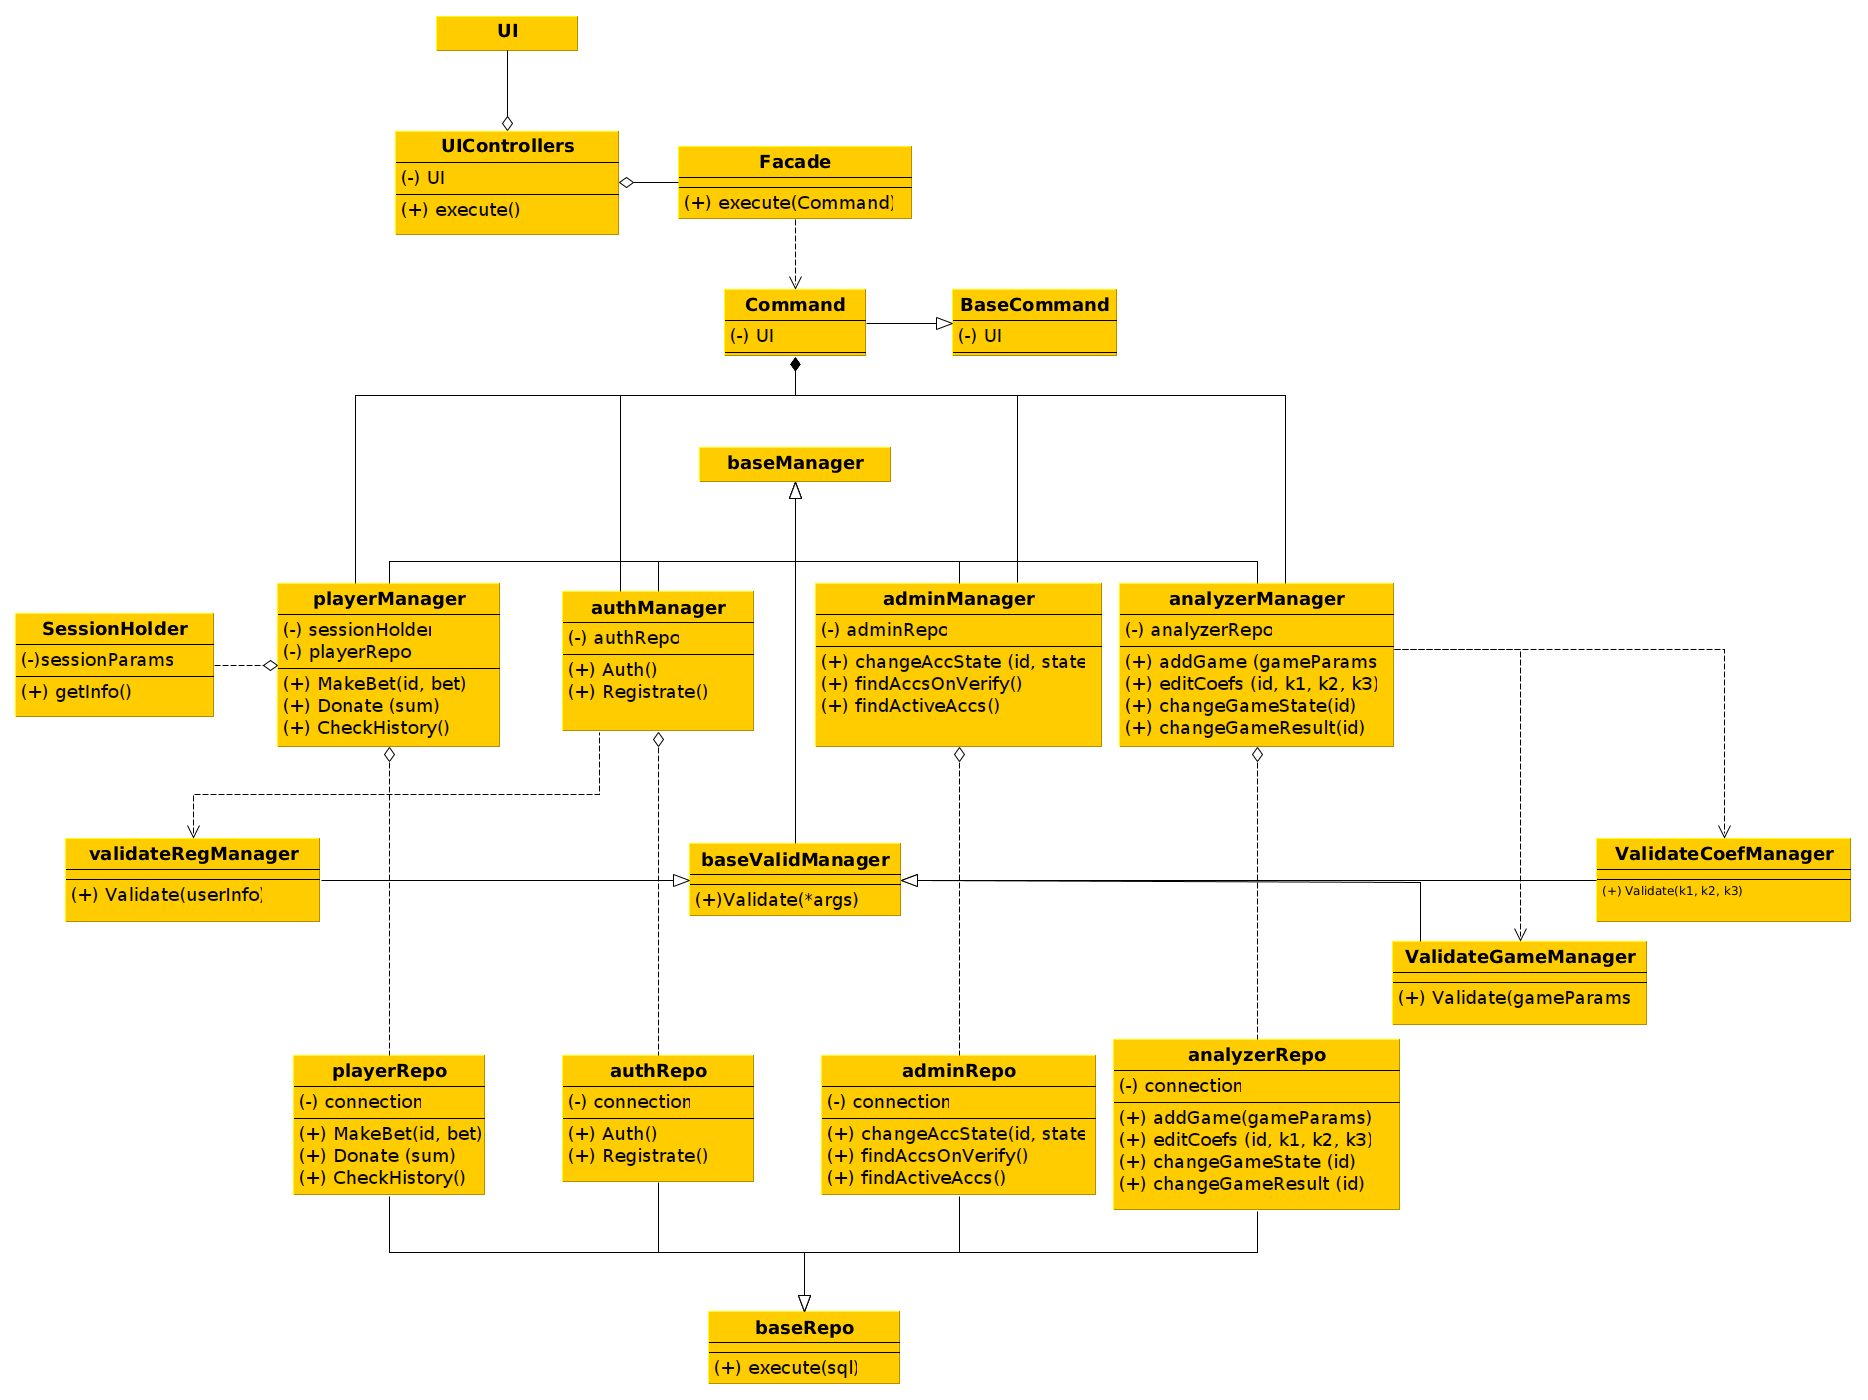
\includegraphics[angle=90, width=\linewidth, height=16cm]{inc/uml.png}
	\end{center}
	\caption{UML-диаграмма классов}
	\label{fig::uml}
\end{figure}
\FloatBarrier

\subsection{Алгоритм работы программы при авторизации пользователя}
Авторизация пользователя происходит при активном взаимодействии с базой данных.

В первую очередь требуется проверить, что логин существует в базе данных. 
Для этого достаточно найти одно значение логина в базе, при этом гарантируется, что поле логина уникальное, и логин присутствует в единственном экземпляре.

После соответствия требуется проверить соответствие введенного пароля и пароля в системе. 
Если они совпадают, то можно выполнить вход в систему, иначе вывести сообщение об ошибке.

При входе системы требуется также получить из БД роль, соответствующий аккаунту, в который входит пользователь.
Для аналитика и администратора в дальнейшем загружается UI, но для игрока требуется провести несколько дополнительных действий.

Во-первых, требуется выгрузить из БД всю основную информацию о пользователе, и кэшировать её.
Это нужно для того, чтобы в дальнейшем не обращаться к БД для проверки параметров (например, хватает ли у пользователя средств для совершения ставки), что снижает время работы с самой базой данных.
Во-вторых, требуется проверить, какой статус у аккаунта. 
Если у пользователя заблокированный аккаунт, то он не может выполнять никаких действий, поэтому требуется в UI заблокировать все соответствующие элементы.

\newpage
На рисунке 5 представлена схема алгоритма работы программы при авторизации:
\FloatBarrier
\begin{figure}[h]	
	\begin{center}
		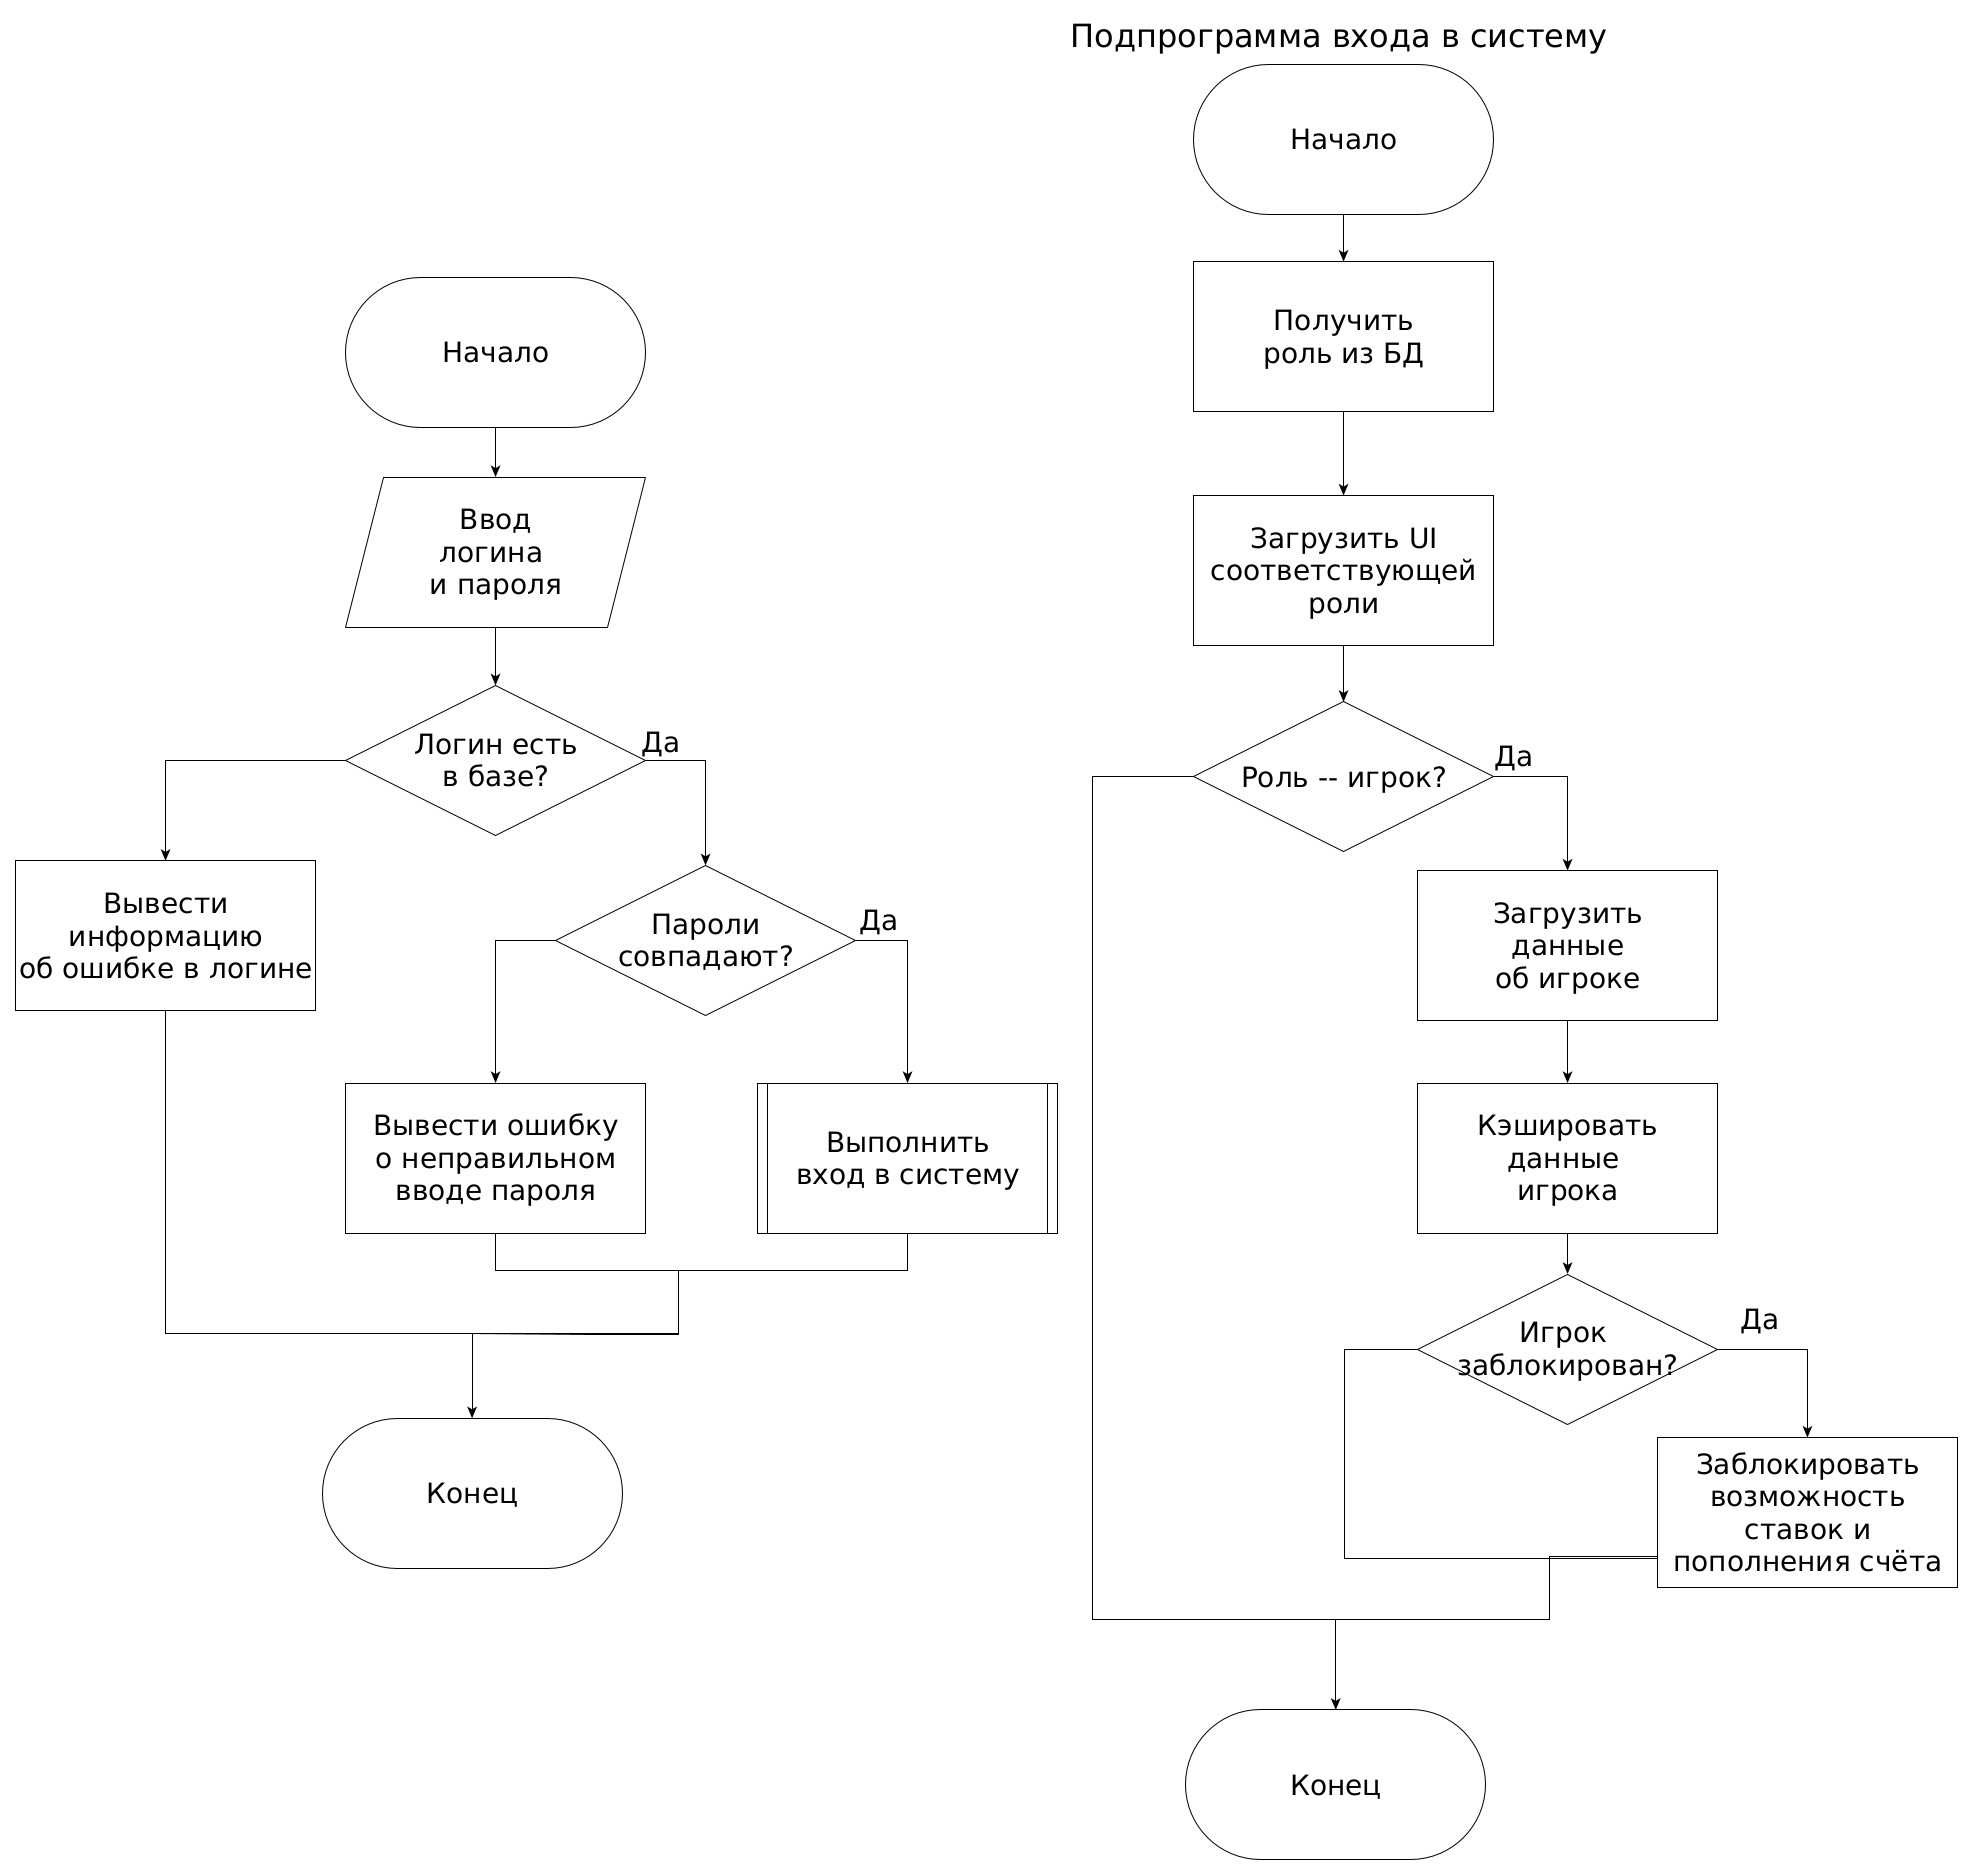
\includegraphics[width=\linewidth]{inc/auth.png}
	\end{center}
	\caption{Схема алгоритма работы программы при авторизации}
	\label{fig::auth}
\end{figure}
\FloatBarrier

\newpage
\subsection{Алгоритм работы при обновлении состояния матча}
Алгоритм работы при обновлении состояния матча является важнейшим для работы системы, так как расчёт выплат по ставкам производится по окончанию матча.

Для автоматического обновления баланса пользователей требуется разработать триггер.
Он будет навешан на таблицу Bet, но сложность заключается в том, что баланс находится в другом отношении -- Account.
Следовательно, требуется вызывать подпрограмму для обновления баланса пользователей.

Также для определения результата матча требуется реализовать собственную функцию, так как в таблице хранится текущий счёт встречи: в таблице нельзя отдельно хранить результат из-за того, что тогда возникнет избыточность в базе, а счёт требуется для корректной оценки пользователем действий в матче. 

Для обновления статуса ставок требуется сравнить результат, выбранный игроком, и реальный. 
Статус ставки хранится в виде целочисленного флага: 1 соответствует выигрышу, 0 -- проигрышу.

Для последовательного прохода по id требуется реализовать курсор, так как требуется изменять баланс пользователей построчно, последовательно итерируясь по всем пользователям, делавших ставки на конкретное событие.

\newpage
На рисунке 6 представлена схема алгоритма обновления состояния матча:
\FloatBarrier
\begin{figure}[h]	
	\begin{center}
		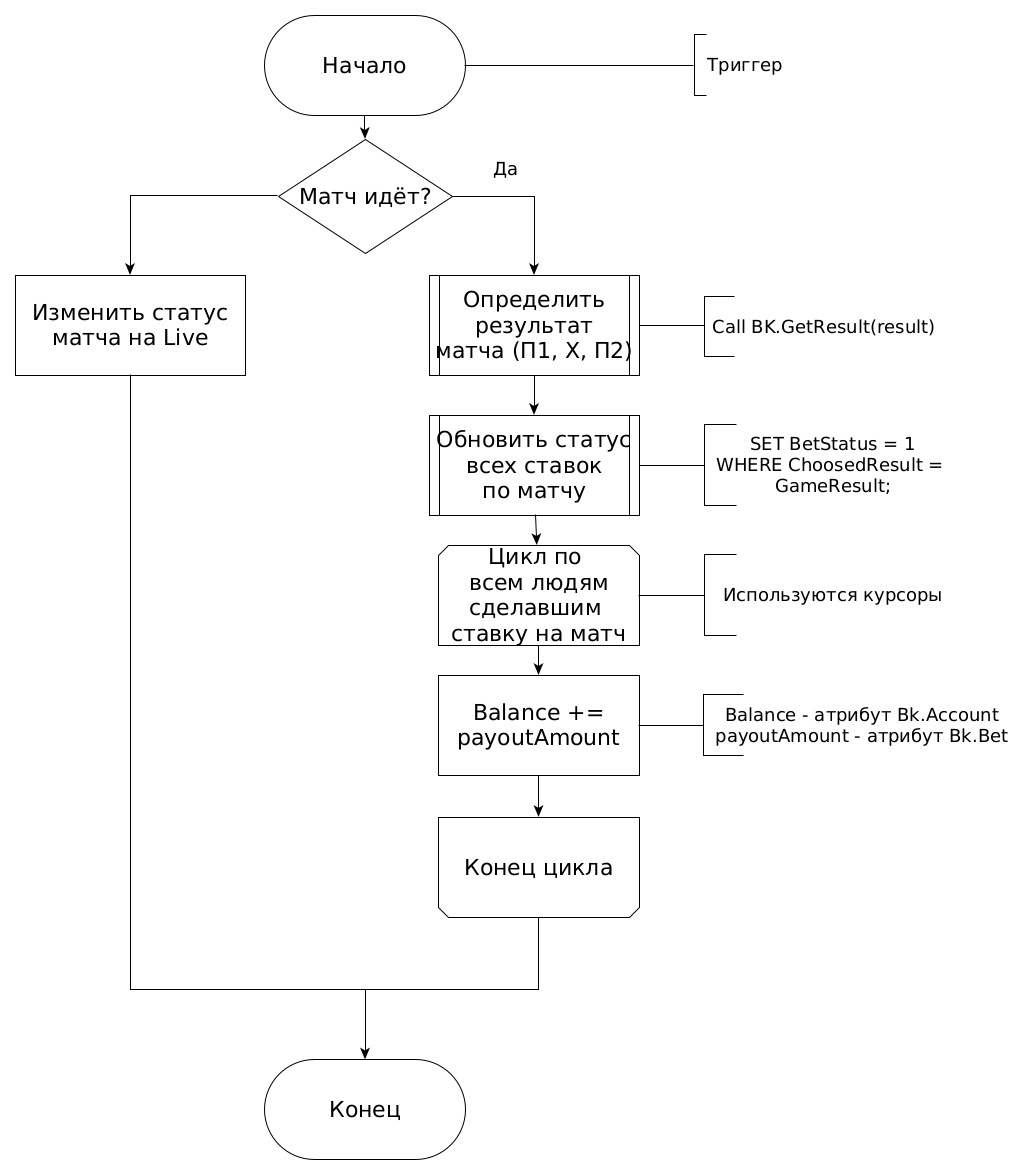
\includegraphics[height=18cm, width=\linewidth]{inc/updateFlow.png}
	\end{center}
	\caption{Схема алгоритма обновления состояния матча}
	\label{fig::update}
\end{figure}
\FloatBarrier

	\section{Технологический раздел}
В этом разделе будет проведен выбор средств реализации ПО, будут приведены листинги кода и демонстрация работы программы.

\subsection{Средства реализации программного обеспечения}
\subsubsection{Выбор языка программирования}
В качестве языка программирования для реализации платформы был выбран Python 3.9, так как имеется опыт разработки проектов на этом языке. 
Также данный ЯП поддерживает парадигму ООП, соответственно, даёт возможность реализовать структуру приложения, приведённую в конструкторской части.

\subsubsection{Выбор СУБД}
В качестве СУБД был выбран PostgreSQL.

Postgres \cite{postgresql} -- это свободно распространяемая объектно-реляционная система управления базами данных.
Данная СУБД предназначена для обработки ряда рабочих нагрузок, от отдельных компьютеров до хранилищ данных или веб-сервисов с множеством одновременных пользователей. 

Выбор обусловлен тем, что имеется опыт разработки проектов с данной СУБД, а также тем, что Python и PostgreSQL являются совместимыми технологиями  \cite{psycopg2}.

\subsubsection{Выбор ПО для графического интерфейса}
В качестве ПО для реализации UI был выбран среда QT по следующим причинам:
\begin{enumerate}
	\item Qt предоставляет широкую поддержку для взаимодействия с Python приложениями.
	\item Qt является программной средой для реализации Desktop-приложений. Пользователь может воспользоваться ПО QtDesigner для разработки UI.
	\item Структура приложений QT позволяет внедрить их в ООП-архитектуру.
	\item У автора есть опыт разработки проектов с использованием QT.
\end{enumerate} 

\subsection{Листинги кода}

\subsubsection{Создание базы данных}
В работе была реализована база данных, соответствующая разработанной в аналитическом и конструкторских разделах.
Помимо создания таблиц, требуется наложить на каждую ограничения.
Были добавлены следующие ограничения:
\begin{itemize}
	\item \textbf{Account} -- баланс игрока должен быть положительным, игроку должно быть не меньше 18 лет, номер паспорта должен состоять из 10 символов, без пробелов;
	\item \textbf{Games} -- корректные коэффициенты (больше 1), сумма вероятностей событий с учётом маржи не меньше, чем 1;
	\item \textbf{Bet} -- сумма ставки от 10 до 1000 у.е, коэффициент больше 1;
	\item \textbf{Users} -- логин и пароль должны состоять как минимум из 5 символов.
\end{itemize} 

Код создания всех таблиц в базе данных с указанием типов атрибутов представлен в приложении А.

Код создания ограничений на таблицы представлен в приложении Б.

\subsubsection{Функции, хранимые процедуры и триггеры}
Всего в работе было реализовано 10 функций и 11 процедур.

В списке перечислены реализованные процедуры и функции:
\begin{itemize}
	\item \textbf{BK.viewTeams(myTeamName text)} -- функция, возвращает команды, доступные для добавления в матч;
	\item \textbf{BK.verifyAccs(surnameString text)} -- функция, возвращает список аккаунтов, которые ждут аутентификации. Аргумент функции соответствует фамилии, по которой требуется производить поиск;
	\item \textbf{BK.getUserInfo(webUserLog text)} -- функция, возвращает полную информацию об пользователе;
	\item \textbf{BK.auth(login text, password text)} -- функция, проверяющая, есть ли аккаунт с логином и паролем в процессе авторизации;
	\item \textbf{BK.findLogin(login text)} -- функция, проверяющая наличие логина в таблице Account;
	\item \textbf{BK.viewGamesAnalyze(name text)} -- функция, возвращающая актуальную линию событий;
	\item \textbf{BK.GetResult(id int)} -- функция, возвращающая победителя матча;
	\item \textbf{BK.GetBetHistory(id int)} -- функция, возвращающая историю ставок по пользователю;
	\item \textbf{BK.GetROI(id int)} -- функция, возвращающая общую доходность пользователя;
	\item \textbf{BK.GetAllActiveAccs()} -- функция, которая возвращает все активные аккаунты в системе;
	\item \textbf{BK.insertUsers(args)} -- процедура, которая добавляет пользователя в таблицу Users;
	\item \textbf{BK.insertAccount(args)} -- процедура добавления нового игрока в таблицу Account;
	\item \textbf{BK.registrate(args)} -- процедура регистрации игрока в систему;
	\item \textbf{BK.updateStatus(id int, status text)} -- процедура изменения статуса аккаунта;
	\item \textbf{BK.addGame(args)} -- процедура добавления нового матча в систему;
	\item \textbf{BK.changeGameState(id int)} -- процедура изменения статуса матча;
	\item \textbf{BK.changeGameResult(id int, result text)} -- процедура изменения счёта матча;
	\item \textbf{BK.changeGameCoef(args)} -- процедура изменения коэффициентов для конкретного матча;
	\item \textbf{BK.MakeBet(args)} -- процедура совершения ставки;
	\item \textbf{BK.Donate(id INT, value float)} -- процедура пополнения баланса игроком.
	\item \textbf{BK.UpdateBalance(id int)} -- процедура платежа клиентам выигранной суммы после завершения матча.
\end{itemize}

На листинге 1 представлен код получения таблицы матчей в текущей линии:
\FloatBarrier
\begin{lstinputlisting}[language=SQL, caption=Получение таблицы матчей в текущей линии, linerange = {78-101},
	basicstyle=\footnotesize\ttfamily, frame=single, breaklines=true]{src/db/sql/functions.sql}
\end{lstinputlisting}
\FloatBarrier

\newpage
На листинге 2 представлен код расчёта итога события:
\FloatBarrier
\begin{lstinputlisting}[language=SQL, caption=Расчёт итога события, linerange = {127-151},
	basicstyle=\footnotesize\ttfamily, frame=single,breaklines=true]{src/db/sql/functions.sql}
\end{lstinputlisting}
\FloatBarrier

\subsubsection{Триггеры}
Триггеры в программе позволяют автоматизировать процесс денежных выплат при выполнении ставки игроком и при расчёте выплаты игрокам по окончанию события.

Было разработано два триггера:
\begin{enumerate}
	\item \textbf{BK.MakeBet()} -- триггер, который списывает с баланса игрока сумму, равную размеру ставки, при заключении пари с БК. Триггер обновляет таблицу Account при добавлении новой записи в таблицу Bet.
	\item \textbf{BK.UpdateBet()} -- триггер, который обновляет баланс всех игроков, которые ставили на только что завершённое событие. Триггер обновляет таблицы Account и Bet при изменении таблицы Games.
\end{enumerate}

На листинге 3 представлен код триггера UpdateBet, связанным с изменением состояния матча:
\FloatBarrier
\begin{lstinputlisting}[language=SQL, caption=Триггер на обновление таблицы Games, linerange = {24-50},
	basicstyle=\footnotesize\ttfamily, frame=single,breaklines=true]{src/db/sql/triggers.sql}
\end{lstinputlisting}
\FloatBarrier

\newpage
На листинге 4 представлен код процедуры обновления баланса пользователей BK.UpdateBalance(id int), которая вызывается внутри триггера UpdateBet:
\FloatBarrier
\begin{lstinputlisting}[language=SQL, caption=Обновление балансов пользователй, linerange = {112-134},
	basicstyle=\footnotesize\ttfamily, frame=single,breaklines=true]{src/db/sql/procedures.sql}
\end{lstinputlisting}
\FloatBarrier

\newpage
\subsubsection{Ролевая модель на уровне БД}
В соответствии с ролевой моделью, были созданы следующие роли:
\begin{enumerate}
	\item \textbf{Client} -- роль, связанная с игроком. Игрок обладает правами на доступ к таблице матчей и ставок, так как он должен совершать ставки и видеть список матчей.
	\item \textbf{Administrator} -- роль, связанная с администратором. Ему выданы полные права на таблицы Users, Account и Bet. Наличие последней обусловлено тем, что администратор имеет возможность увидеть доходность активных пользователей, чтобы заблокировать прибыльных игроков.
	\item \textbf{Analyzist} -- роль, связанная с аналитиком. Он обладает доступом к таблицам Teams, Games и Bet.
\end{enumerate}

На листинге 5 представлен код выдачи прав по ролям:
\FloatBarrier
\begin{lstinputlisting}[language=SQL, caption=Выдача прав ролям, 
	basicstyle=\footnotesize\ttfamily, frame=single,breaklines=true]{src/db/sql/roles.sql}
\end{lstinputlisting}
\FloatBarrier

\newpage
\subsubsection{Приложение}
Все действия, которые приложение может выполнить, обернуты в SQL функции, которые затем вызываются классами, ответственными за взаимодействие с базой данных.

На листинге 6 представлен код выполнения SQL-запроса в Python:
\FloatBarrier
\begin{lstinputlisting}[language=Python, caption=Выполнение SQL-запроса, linerange = {11-28},
	basicstyle=\footnotesize\ttfamily, frame=single,breaklines=true]{src/db/baseRepo.py}
\end{lstinputlisting}
\FloatBarrier

На листинге 7 представлен код пополнения баланса пользователя:
\FloatBarrier
\begin{lstinputlisting}[language=Python, caption=Пополнение баланса пользователя, linerange = {44-47},
	basicstyle=\footnotesize\ttfamily, frame=single,breaklines=true]{src/db/playerRepo.py}
\end{lstinputlisting}
\FloatBarrier

\newpage
\subsection{Демонстрация работы программы}
В этом разделе будут показана демонстрация работы программы при выполнении основных действий для каждой из представленных в программе ролей. 

\subsubsection{Вход в систему}
Стартовый экран приложения представлен на рисунке \ref{fig::start}. 
Пользователь может войти в систему, введя логин и пароль в специальном поле.
Также отсюда можно перейти к регистрации

\FloatBarrier
\begin{figure}[hp]	
	\begin{center}
		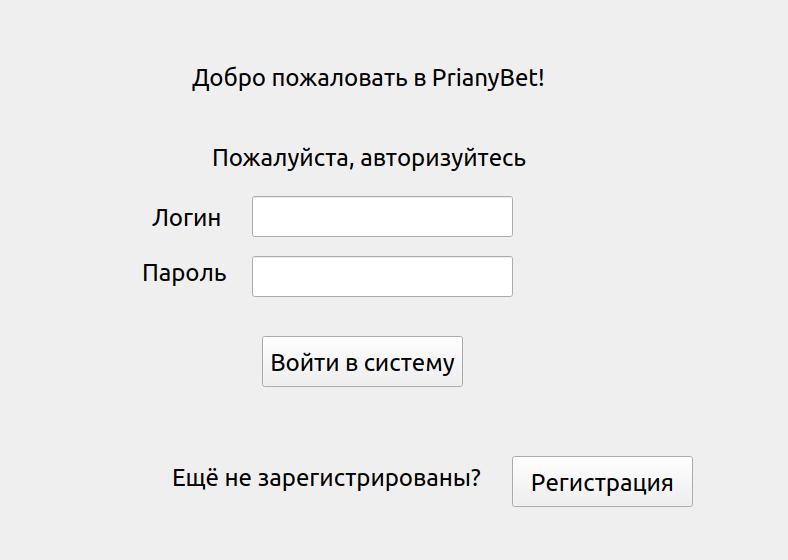
\includegraphics[width=\linewidth]{inc/start.png}
	\end{center}
	\caption{Стартовый экран приложения}
	\label{fig::start}
\end{figure}
\FloatBarrier

\newpage
\subsubsection{Регистрация}
Экран регистрации представлен на рисунке \ref{fig::reg}. 
Пользователь вводит все данные, которые после ввода проверяются программой.
В случае успеха пользователь регистрируется в системе, либо же система выведет сообщение об ошибке.

\FloatBarrier
\begin{figure}[hp]	
	\begin{center}
		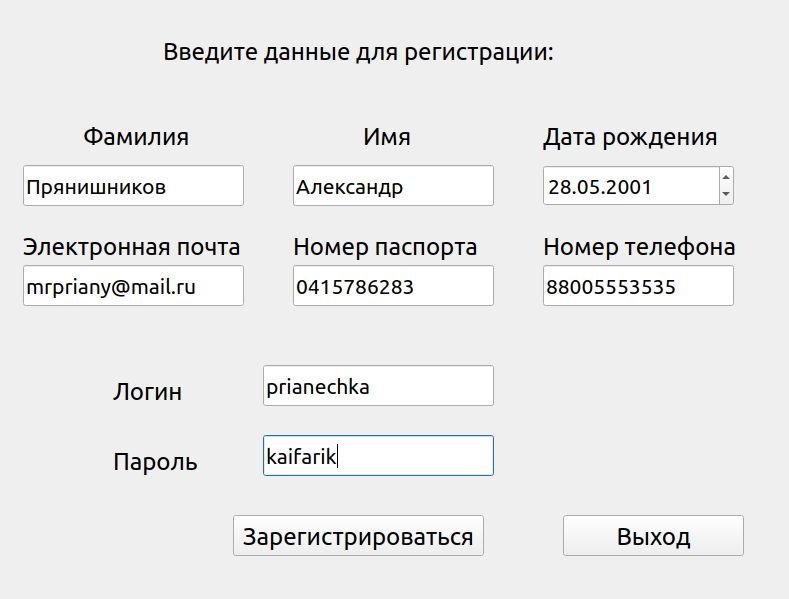
\includegraphics[width=\linewidth]{inc/registrate.png}
	\end{center}
	\caption{Экран регистрации}
	\label{fig::reg}
\end{figure}
\FloatBarrier

\newpage
\subsubsection{Стартовое меню игрока}
Стартовый экран игрока представлен на рисунке \ref{fig::user}. 
Игрок может посмотреть сверху свои данные: баланс, логин, а также статус аккаунта.
С этого экрана можно перейти к просмотру истории ставок, пополнению баланса или непосредственно к выполнению ставок.

\FloatBarrier
\begin{figure}[h]	
	\begin{center}
		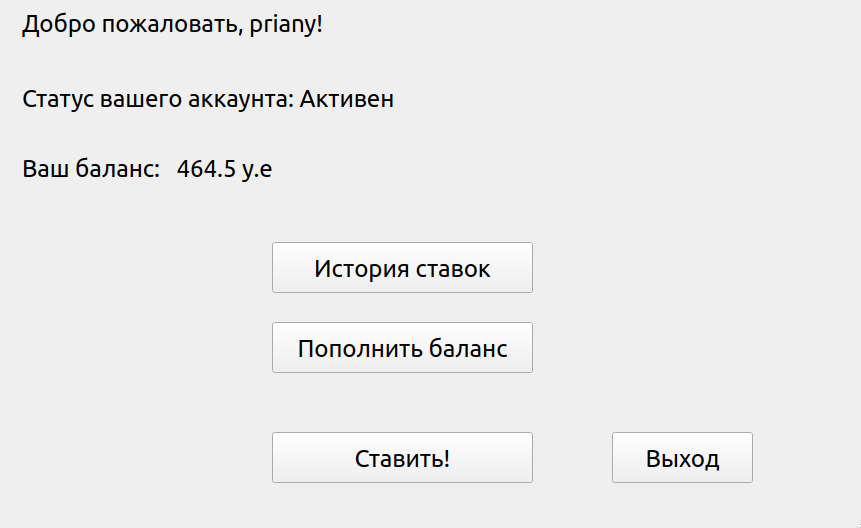
\includegraphics[width=\linewidth]{inc/user.png}
	\end{center}
	\caption{Стартовый экран игрока}
	\label{fig::user}
\end{figure}
\FloatBarrier

\subsubsection{Пополнение баланса}
Экран пополнения баланса представлен на рисунке \ref{fig::balance}. 
Игрок выбирает сумму пополнения, после чего при нажатии кнопки пополнения баланс успешно пополняется.

\FloatBarrier
\begin{figure}[h]	
	\begin{center}
		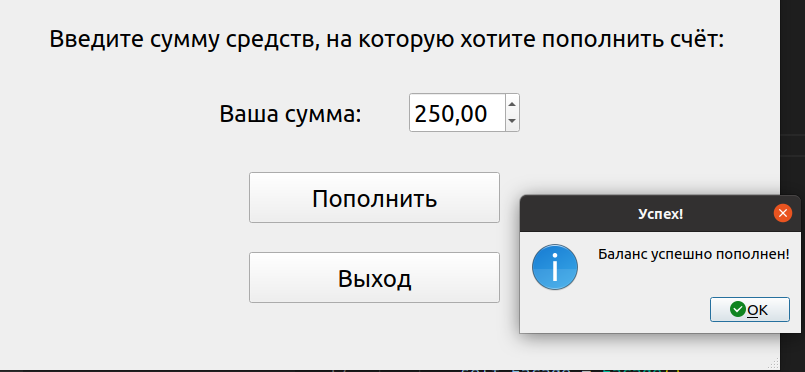
\includegraphics[height = 6cm, width=\linewidth]{inc/balance.png}
	\end{center}
	\caption{Экран пополнения баланса}
	\label{fig::balance}
\end{figure}
\FloatBarrier

\subsubsection{Выполнение ставок}
Экран выполнения ставок представлен на рисунке \ref{fig::bet}.

Игрок может увидеть в таблице все события, которые присутствуют в линии в данный момент.
Для выбора события, на которое нужно сделать ставку, пользователь должен выделить строку с нужным событием.
Слева внизу игрок может выбрать событие для ставки, а также сумму, на которую он хочет заключить пари.

После нажатия кнопки выполнения ставки программа оценит валидность введённых данных, и, в случае успеха, выдаст информационное сообщение.

\FloatBarrier
\begin{figure}[h]	
	\begin{center}
		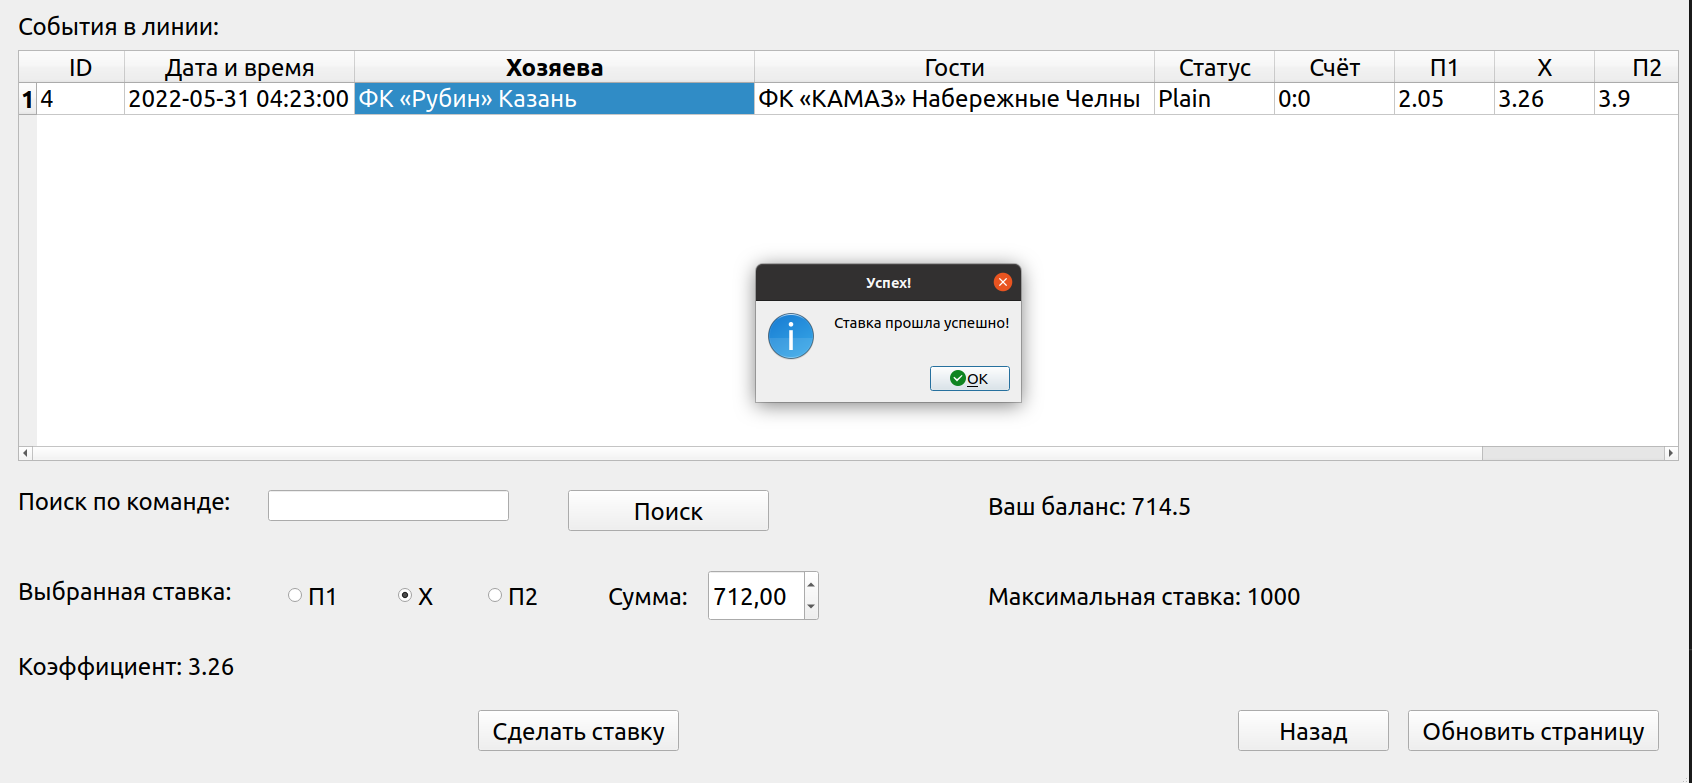
\includegraphics[height = 7cm, width=\linewidth]{inc/bet.png}
	\end{center}
	\caption{Экран выполнения ставок}
	\label{fig::bet}
\end{figure}
\FloatBarrier

\subsubsection{Просмотр истории ставок}
Экран просмотра истории ставок представлен на рисунке \ref{fig::history}.

Игрок может увидеть в таблице все события, которые присутствуют в линии в данный момент.
Для выбора события, на которое нужно сделать ставку, пользователь должен выделить строку с нужным событием.
Слева внизу игрок может выбрать событие для ставки, а также сумму ставки.

После нажатия кнопки выполнения ставки программа оценит валидность введённых данных, и, в случае успеха, выдаст информационное сообщение.

\FloatBarrier
\begin{figure}[h]	
	\begin{center}
		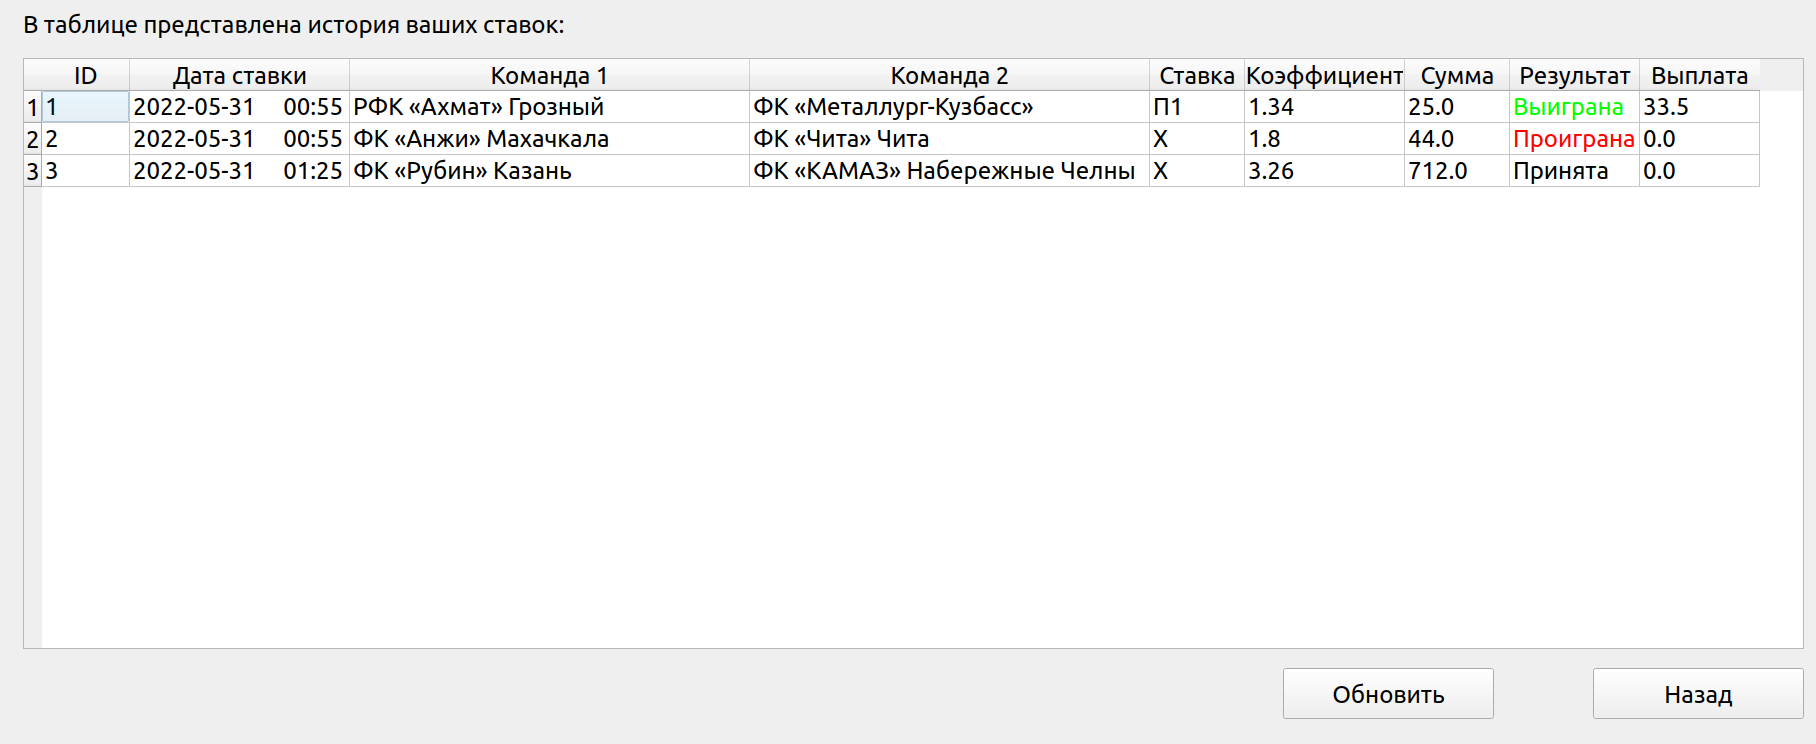
\includegraphics[width=\linewidth]{inc/history.png}
	\end{center}
	\caption{Экран просмотра истории ставок}
	\label{fig::history}
\end{figure}
\FloatBarrier

\subsubsection{Добавление матчей в линию аналитиком}
Экран добавления матчей в линию представлен на рисунке \ref{fig::add}.

Экран доступен только в случае входа аналитика в приложение из стартового окна.
В таблице представлен список клубов, доступных для добавления в событие.
Можно воспользоваться кнопкой поиска для нахождения клубов.
Выбор команды осуществляется нажатием на название мышкой.

Также внизу аналитик должен выбрать вероятности наступления событий. 
Сумма вероятностей должна быть равна 100\%.

\FloatBarrier
\begin{figure}[h]	
	\begin{center}
		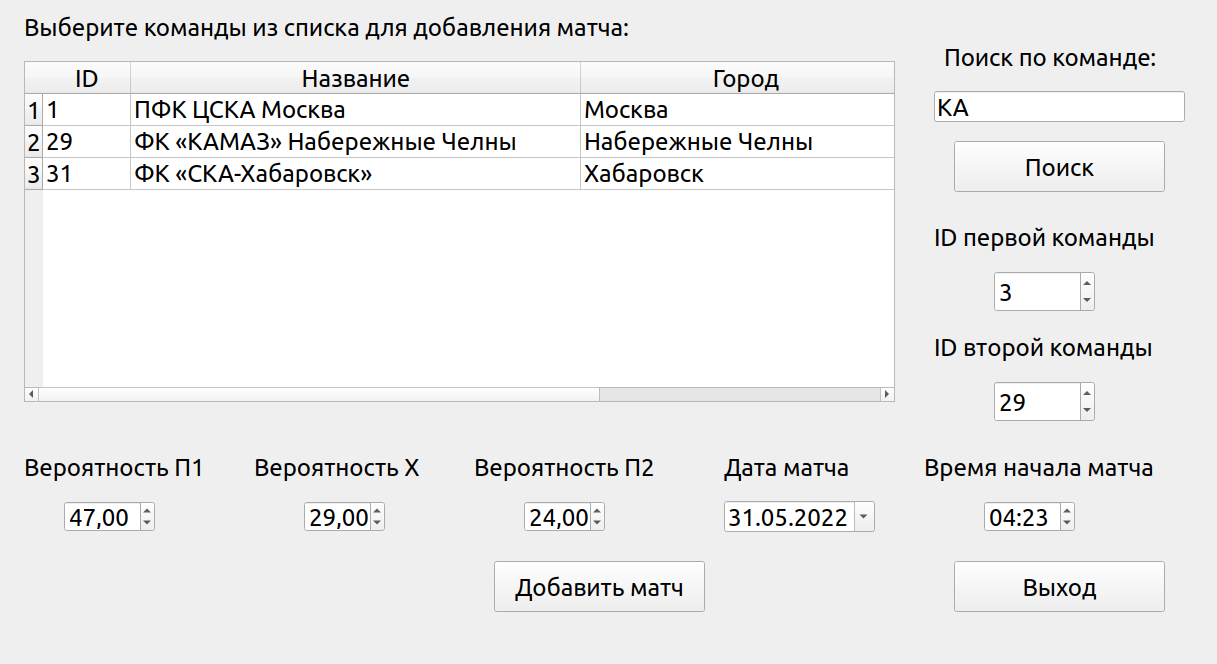
\includegraphics[width=\linewidth]{inc/addMatch.png}
	\end{center}
	\caption{Экран добавления матчей в линию}
	\label{fig::add}
\end{figure}
\FloatBarrier

\subsubsection{Экран изменения матчей}
Экран изменения матчей в линии представлен на рисунке \ref{fig::change}.

Экран доступен только в случае входа аналитика в приложение из стартового окна.
В таблице представлены матчи, добавленные аналитиком в предыдущем окне.
Для изменения состояния матча или изменения счёта нужно нажать на строку с событием, а затем нажать на требуемую кнопку внизу таблицы.

Также внизу аналитик может изменить вероятности наступления событий.

\FloatBarrier
\begin{figure}[h]	
	\begin{center}
		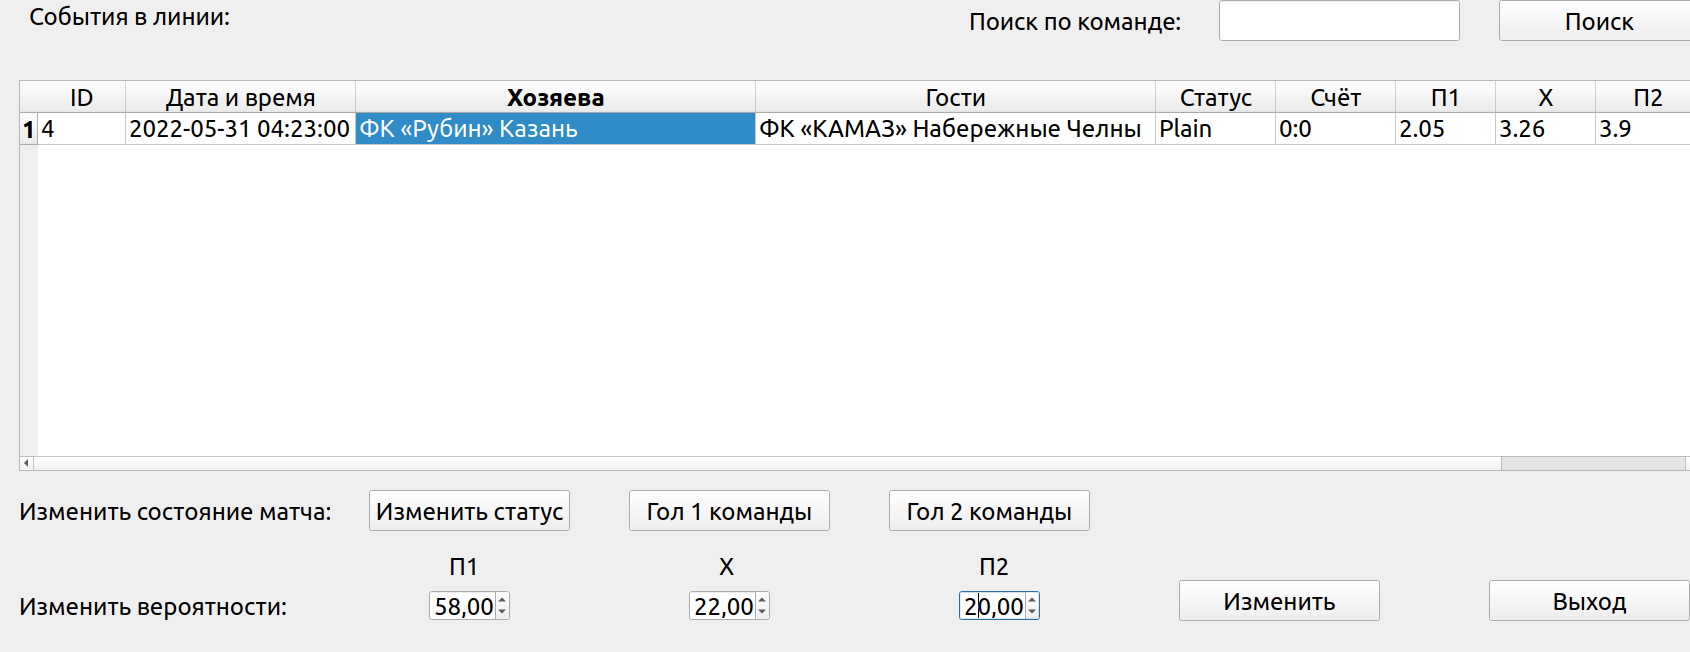
\includegraphics[height=6cm, width=\linewidth]{inc/matches.png}
	\end{center}
	\caption{Экран изменения матчей в линию}
	\label{fig::change}
\end{figure}
\FloatBarrier

\subsubsection{Экран верификации пользователей}
Экран верификации пользователей в линии представлен на рисунке \ref{fig::verify}.

Экран доступен только в случае входа администратора в приложение из стартового окна.
Аналитик в таблице видит список аккаунтов, которые требуют верификации.
В зависимости от введённых данных аналитик может либо верифицировать аккаунт, либо заблокировать.

\FloatBarrier
\begin{figure}[h]	
	\begin{center}
		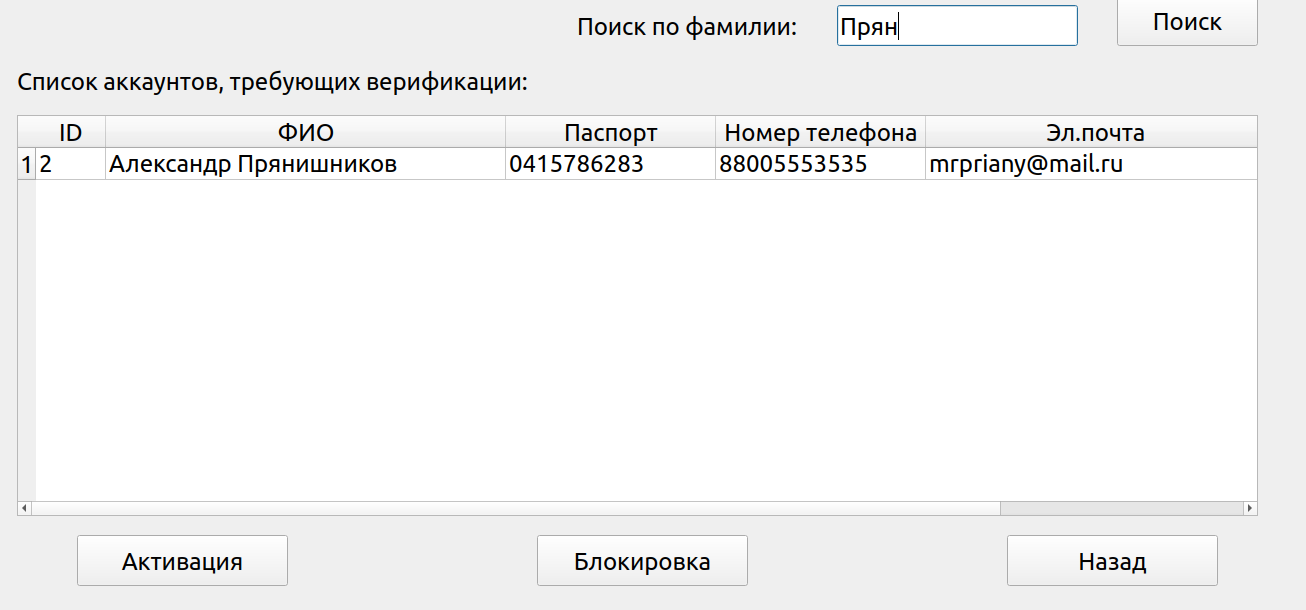
\includegraphics[width=\linewidth]{inc/verify.png}
	\end{center}
	\caption{Экран верификации пользователей}
	\label{fig::verify}
\end{figure}
\FloatBarrier
	\section{Экспериментальный раздел}
В этом разделе будут продемонстрированы результаты тестирования разработанного ПО.
Будет приведена таблица результатов измерений зависимости времени ответа базы данных от индексации столбцов.
Будет отражён график, отображающий зависимость времени ответы от индексации.
Будут приведены технические характеристики устройства, на котором производилось тестирование.

\subsection{Технические характеристики}
Технические характеристики устройства, на котором выполнялось тестирование, следующие:
\begin{itemize}
	\item операционная система: Ubuntu 20.04.1 LTS \cite{ubuntu};
	\item тип системы: 64-битная;
	\item память: 8 GB;
	\item процессор: Intel Core i5-1135G7 @ 2.40GHz \cite{intel}.
	\item количество ядер процессора: 8.
	\item ёмкость диска: 512 GB;
\end{itemize}

Во время тестирования ноутбук был нагружен только встроенными приложениями окружения, а также непосредственно системой тестирования. 
Сторонние приложения запущены не были.

\subsection{Зависимость времени ответа базы данных от индексации}
Требуется оценить зависимость времени ответа базы данных от индексации и размера таблицы.

Оценка будет производиться для таблицы Games, так как она является самой востребованной -- её просматривают все игроки, и её обновление происходит в реальном времени. 
Измеряться будет время ответа от функции, которая возвращает актуальную линию. 
Индексироваться будет поле team1ID, связанное c ID одной из команд.

В таблице 1 представлены результаты тестов. Время -- в миллисекундах.
\FloatBarrier
\begin{table}[h]
	\caption{Результаты тестов}
	\centering
	\begin{tabular}{ | l | l | l |}
		\hline
		Кол-во записей в БД & Без индексации & С индексацией \\ 
		\hline
		10 & 34 & 30 \\
		30 & 41 & 33 \\
		50 & 43 & 37 \\
		100 & 55 & 39 \\
		200 & 70 & 44 \\
		400 & 81 & 55 \\
		600 & 91 & 69 \\
		800 & 98 & 79 \\
		1000 & 112 & 91 \\
		\hline
	\end{tabular}
\end{table}
\FloatBarrier

На рисунке 16 представлен график, иллюстрирующий таблицу:
\FloatBarrier
\begin{figure}[h]	
	\begin{center}
		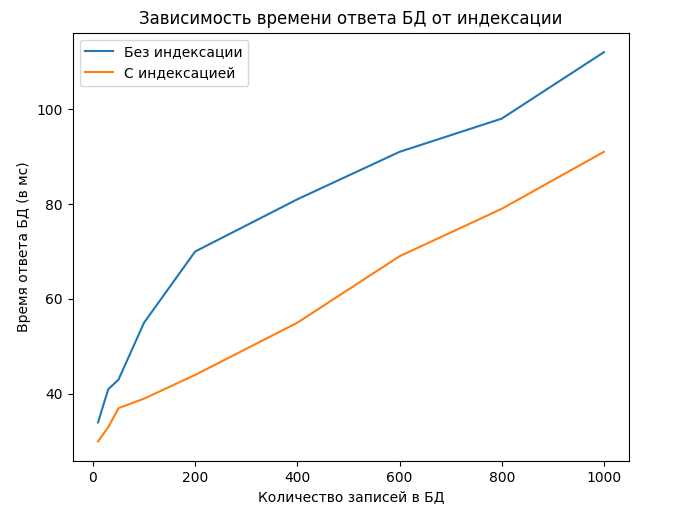
\includegraphics[height=10cm, width=\linewidth]{inc/graph.png}
	\end{center}
	\captionsetup{justification=centering, labelsep=defffis}
	\caption{График зависимости времени ответа БД от индексации}
\end{figure}
\FloatBarrier

Как видно, индексация позволила уменьшить время ответа. При $N=600$ время сократилось на $30\%$, при $N=800$ -- на $20\%$. При этом индексированная таблица возвращала результат быстрее при всех измерениях.
	
	\chapter*{Заключение}
В рамках курсового проекта было создано ПО для обеспечения работы букмекерской конторы.

Была спроектирована предметная база данных.
Было написано 10 функций, 11 процедур и два триггера, включающие внутри себя сложные аналитические запросы. 
Была выделена ролевая модель как на уровне БД, так и на уровне приложения. 
Была исследована зависимость быстродействия БД от индексации таблицы.

Также в работе были выполнены следующие задачи:
\begin{itemize}
	\item проведена формализация задачи и определен требуемый функционал;
	\item проведён анализ СУБД и описана структуру БД, включая объекты, из которых она состоит;
	\item создана и заполнена БД;
	\item создан программный продукт для решения задачи, реализованы выбранные алгоритмы;
	\item реализован понятный интерфейс для клиента.
\end{itemize}
	
	\addcontentsline{toc}{section}{СПИСОК ИСПОЛЬЗОВАННЫХ ИСТОЧНИКОВ}
	\renewcommand\bibname{СПИСОК ИСПОЛЬЗОВАННЫХ ИСТОЧНИКОВ}
	\begingroup
	\renewcommand{\anonsection}[2]{}
	\begin{thebibliography}{}
		\bibitem{bk}
		Федеральный закон от 29.12.2006 N 244-ФЗ (последняя редакция) «О государственном регулировании деятельности по организации и проведению азартных игр и о внесении изменений в некоторые законодательные акты Российской Федерации» // Собрание законодательства РФ,  29.12.2006. – N 244. – Ст.6.
		
		\bibitem{bk2}
		Федеральный закон от 07.08.2001 N 115-ФЗ (последняя редакция) «О противодействии легализации (отмыванию) доходов, полученных преступным путем, и финансированию терроризма» // Собрание законодательства РФ,  07.08.2001. – N 115. – Ст.7.
		
		\bibitem{postgresql}
		PostgreSQL: Документация. [Электронный ресурс]. – Режим доступа: 
		\url{https://postgrespro.ru/docs/postgresql/} свободный – (31.05.2022).
		
		\bibitem{kfs}
		Matthew Zhou «Optimal Bookmaking» // European Journal of Operational Research. 2021 Vol. 285. P. 10.
		
		
		\bibitem{dbms}
		Когаловский М.Р. «Энциклопедия технологий баз данных.» — М.: Финансы и статистика, 2002. — 800 с.
		
		\bibitem{psycopg2}
		Psycopg – PostgreSQL database adapter for Python [Электронный ресурс]. – Режим доступа: 
		\url{https://www.psycopg.org/docs/} свободный – (31.05.2022).
		
		\bibitem{ubuntu}
		Ubuntu 20.04.3 LTS (Focal Fossa) [Электронный ресурс]. – Режим доступа: 
		\url{https://releases.ubuntu.com/20.04/} свободный – (31.05.2022).
		
		\bibitem{intel}
		Процессор Intel® Core™ i5-1135G7 [Электронный ресурс]. – Режим доступа: 
		\url{https://www.intel.ru/content/www/ru/ru/products/sku/208658/intel-core-i51135g7-processor-8m-cache-up-to-4-20-ghz/specifications.html} свободный – (31.05.2022).

	\end{thebibliography}
	\endgroup
	\newpage
	\anonsection{ПРИЛОЖЕНИЕ А}
	На листинге 8 представлен код создания таблиц базы данных, перечисленных в конструкторском разделе.
	\FloatBarrier
	\begin{lstinputlisting}[language=SQL, caption=Создание таблиц в БД, 
		basicstyle=\footnotesize\ttfamily, frame=single,breaklines=true]{src/db/sql/create.sql}
	\end{lstinputlisting}
	\FloatBarrier
	
	\clearpage
	
	\anonsection{ПРИЛОЖЕНИЕ Б}
	\FloatBarrier
	\begin{lstinputlisting}[language=SQL, caption=Создание ограничений на таблицы, 
		basicstyle=\footnotesize\ttfamily, frame=single,breaklines=true]{src/db/sql/constraints.sql}
	\end{lstinputlisting}
	\FloatBarrier
	%\bibliographystyle{utf8gost705u} 
	%\bibliography{source}
\end{document}